%=============================================================================
% Tesis de Licenciatura: .....
%=============================================================================
   
%=============================================================================
%                                Preambulo Latex
%=============================================================================
\documentclass[oneside,letterpaper,10pt, spanish]{report}

\usepackage[spanish]{babel} % division de silabas en español.

\usepackage[T1]{fontenc}
\usepackage[utf8]{inputenc} %%%Para poner acentos directamente


\usepackage{babel}
\setcounter{secnumdepth}{3} 
\setcounter{tocdepth}{3}  
\usepackage{makeidx}
\usepackage{graphics}  
\usepackage[boxed]{algorithm}
\usepackage{algorithmic}
\usepackage[dvips]{graphicx}
\usepackage{latexsym}
\usepackage{amssymb} 
\usepackage{amsthm}
\usepackage{url}
\usepackage{color}
\usepackage{cite} % para contraer referencias
 \usepackage{enumerate} 
 \usepackage{listings}
 \usepackage{color}
 \usepackage{afterpage}
 
\addtolength{\textwidth}{1cm} % Ancho del texto

% traducción de algunos nombres del paquete algorithm
\floatname{algorithm}{Algoritmo}
\renewcommand{\listalgorithmname}{Indice de algoritmos}

\usepackage{vmargin}

\setpapersize{A4}
\setmargins{2.5cm}       % margen izquierdo
{1.5cm}                        % margen superior
{16.5cm}                      % anchura del texto
{23.42cm}                    % altura del texto
{10pt}                           % altura de los encabezados
{1cm}                           % espacio entre el texto y los encabezados
{0pt}                             % altura del pie de página
{2cm}                           % espacio entre el texto y el pie de página


%parametros para escribir codigo java



\definecolor{dkgreen}{rgb}{0,0.6,0}
\definecolor{gray}{rgb}{0.5,0.5,0.5}
\definecolor{mauve}{rgb}{0.58,0,0.82}
\renewcommand{\lstlistingname}{Código}
\lstset{frame=tb,
	language=Java,
	aboveskip=3mm,
	belowskip=3mm,
	showstringspaces=false,
	columns=flexible,
	basicstyle={\small\ttfamily},
	numbers=left,
	numberstyle=\tiny\color{gray},
	keywordstyle=\color{blue},
	commentstyle=\color{dkgreen},
	stringstyle=\color{mauve},
	breaklines=true,
	breakatwhitespace=true,
	tabsize=4,
	literate={á}{{\'a}}1 {ã}{{\~a}}1 {é}{{\'e}}1,
}

%%%%%%%%%%%%%%%% DEFINICIONES DE ALGUNOS COMANDOS Y AMBIENTES %%%%%%%%%%%%%%%




\newcounter{ruleAGcounter}
\newenvironment{AG}
{
	\setcounter{ruleAGcounter}{0} \begin{center} \begin{figure}[!hb]
			\rule{\textwidth}{.5pt} \footnotesize
		}
		{\normalsize \rule{\textwidth}{.5pt} \end{figure} \end{center}}

\newcommand{\newproduction}[2]{$p_\arabic{ruleAGcounter}$:
	\emph{#1} $\rightarrow$ \emph{#2}
	\addtocounter{ruleAGcounter}{1}\\}

\renewcommand{\labelitemi}{$\bullet$}
\renewcommand{\labelitemii}{$\ast$}
\makeatother
\makeindex

\newcommand{\letraEcore} [1] {\texttt{#1}}


%============================================================================


\begin{document}
	
	
	\title{
		Universidad Nacional de Río Cuarto\\
		$\;$\\
		$\;$\\
		\small{Trabajo de tesis para la obtención del grado de Licenciatura en Ciencias de la Computación}
		$\;$\\$\;$\\
		\Large{\textbf{QVTSInvoker\\
				Automatización y Optimización de la invocación de aplicaciones externas a un Workflow, usando servicios web y transformaciones de modelos.
				 }}
	} 
	
	\author{
		Autores\\
		Jaimez Jacinto \\
		Pereyra Orcasitas Nicolás\\
		\\ \\ \\
		Director de Tesis: \emph{Mg. Marcela Daniele}\\ 
		Co-Director de Tesis: \emph{Mg. Ariel Gonzalez}\\ 
	}
	
	\date{Río Cuarto, Argentina\\ Septiembre 2016}
	
	
	\maketitle
	
%Para dejar una página en blanco
\newpage
\mbox{}
\thispagestyle{empty} % para que no se numere esta página


%\begin{abstract}
\chapter*{Resumen}

\pagenumbering{roman} % para comenzar la numeracion de paginas en numeros romanos
\addcontentsline{toc}{chapter}{Resumen} % si queremos que aparezca en el índice

La tecnología de Web Service (WS) permite invocar aplicaciones externas, por ejemplo desde un motor de workflow y proporcionar beneficios significativos en el Workflow Management System (WFMS). Con el gran número de WS's que proporcionan una funcionalidad similar, es importante encontrar el mejor WS que cumpla con las necesidades del usuario, incluyendo tanto sus requisitos funcionales como los no funcionales. 
La descripción no funcional del Servicio requiere especificar en tiempo de ejecución los atributos de calidad que pueden influir en la elección de un WS ofrecido por un proveedor. En este sentido, es fundamental el uso de métricas para evaluar las características de calidad de los WS's (QoS) con el fin de filtrar los WS's conocidos y obtener el más adecuado.

El comportamiento dinámico de los WS’s en relación con el desarrollo de nuevos servicios y el constante cambio de los existentes requiere un proceso de evaluación continuo, que conduce a capturar información del WS con respecto a su calidad y rendimiento de evaluación conforme a lo solicitado por el workflow. En este trabajo se realiza un refinamiento del proceso de contrastación de WS ofrecidos por proveedores y solicitados por usuarios del workflow, se definen y usan métricas para evaluar los atributos de calidad de dichos servicios, y se propone una herramienta para automatizar este procedimiento de selección de aplicaciones externas al workflow

\emph{Palabras clave}: Web Service o WS, workflow, características de calidad o QoS

\thispagestyle{empty} % para que no se numere esta página
%\end{abstract}

\chapter*{Agradecimientos}
\addcontentsline{toc}{chapter}{Agradecimientos} % si queremos que aparezca en el índice

{\sl Queremos agradecer a todas las personas que han hecho posible la realización de esta tesis. A nuestros directores de tesis Marcela Daniele y Ariel Gonzalez, que han permitido llevar a un final exitoso este trabajo, por su asesoría, dedicación y sus valiosos aportes guiándonos sin ser directivas y mostrando en cada momento una inmejorable disposicón ante las dudas que durante la realización del trabajo nos surgieron, aportando siempre valiosas observaciones que tutelaron esta investigación.} {\sl A nuestras familias y amigos, por su incondicional apoyo durante este largo camino.}

{\sl Además, debemos retribuir con cordial gratitud tanto a la Universidad Nacional de Río Cuarto como a la Facultad de Ciencias Exactas, Físico-Químicas y Naturales, y en especial al Departamento de Computación, por permitirnos desarrollar nuestras formaciones individuales de grado con excelente material académico, pero sobre todo humano durante todos estos años.
}





%\end{flushright}


\listoffigures
\addcontentsline{toc}{chapter}{Lista de figuras} % para que aparezca en el indice de contenidos
%Las siguintes 3 lineas es para sacarle la numeracion de paginas al Indice
%\addtocontents{toc}{\protect\thispagestyle{empty}}
\tableofcontents %put toc in
%\cleardoublepage %start new page






\chapter{Introducci\'on}
\label{Introduccion}



\pagenumbering{arabic} 
\setcounter{page}{1}

La globalización y los cambios de paradigmas empresariales, la evolución de las tecnologías de la información y la política liberal imperante hoy en el mundo, ubican a las organizaciones en el juego de la competitividad internacional. Las iniciativas sobre calidad y la mejora continua de los procesos ya no son suficientes. Se deben considerar nuevos paradigmas empresariales que permitan a las organizaciones obtener mejoras radicales mediante el uso de nuevas y potentes herramientas que faciliten el diseño del trabajo. Las organizaciones se orientan a ser más horizontales hacia el enfoque de redes de procesos, las que deben ser diseñadas de principio a fin, empleando nuevas tecnologías. El cambio radical de procesos comprende la visualización de nuevas estrategias de trabajo, el desarrollo de la propia actividad de diseño del proceso con tecnologías de la información innovadoras y la implementación del cambio en todas sus dimensiones: la tecnológica, la humana y la organizativa, a fin de establecer los mecanismos para un constante crecimiento del valor de las organizaciones. Para lograr un adecuado cambio integral de los procesos, es conveniente confeccionar un mapa de los mismos a fin de determinar los niveles de cambios a realizar. Por lo tanto, la identificación y el modelado de negocio necesario para generar un producto o ejecutar un servicio, es de gran importancia en el desarrollo de cualquier industria. Un conocimiento claro y ordenado de los procesos de negocio facilita su optimización y adaptación. Estas características proporcionan a la organización una gran capacidad de reacción cuando el proceso es automático.	\\	
Un proceso de negocio es un conjunto de tareas relacionadas lógicamente que se ejecuta con la intención de obtener un resultado de negocio particular, el cual incluye recursos humanos así como los recursos materiales con el objetivo de producir un beneficio para la organización. El modelado de procesos de negocio permite visualizar las tareas, actividades y flujos, así como las diferentes unidades organizacionales que son afectadas por el proceso. La ingeniería de procesos de negocio se ha definido como el planteo fundamental y diseño del proceso de negocio para lograr un mejoramiento en las medidas de rendimientos tales como costo, calidad de servicio y velocidad. Estos procesos de negocio se describen y automatizan a través de los Workflow Management System (WFMS) . Los WFMS proporcionan herramientas integradas para automatizar los procesos de negocio, permitiendo a las organizaciones estandarizar y racionalizar las tareas repetitivas, y supervisar el progreso de las mismas, eliminando rutinas en las que es fácil cometer errores. La eliminación de los procesos que consumen tiempo y las costosas rutinas manuales, brinda la posibilidad de conectar al personal con la información y los procesos que necesitan para mejorar los ingresos y recortar los gastos \cite{WfMCa}.\\
Por otra parte, el ambiente donde las organizaciones operan es cada vez más competitivo y agresivo. En estos días, debido a la globalización de los mercados, las compañías tienen que operar “globalmente”, lo cual implica la posibilidad de interoperar unas con otras. En la actualidad existe la Coalición de Administración de Workflow (Workflow Management Coalition - WfMC), fundada en 1993 y con más de 180 miembros en 25 países, la cual está abocada al avance en la tecnología de workflow y su uso en la industria con el propósito de estandarizar en esta materia. El Modelo de Referencia de Workflow, desarrollado por la WfMC, define un marco genérico para la construcción de WFMS, permitiendo la interoperabilidad entre ellos y con otras aplicaciones involucradas. Dicho modelo define cinco interfaces, que permiten a las aplicaciones del workflow la comunicación a distintos niveles. En particular, para permitir la interacción de los usuarios con el motor del workflow utiliza una lista de trabajo, que es manejada por un administrador. La Interfaz de las Aplicaciones de Clientes es la encargada de manejar la interacción entre el motor del workflow y el administrador de la lista de trabajo. Por otro lado, la Interfaz de las Aplicaciones Invocadas se define para la invocación de las aplicaciones externas. La WfMC ha especificado un conjunto de WAPI's (Workflow Aplication Programming Interfaces) para la administración de los Workflow. Estas WAPI's definen las funciones de las interfaces como llamadas a APIs en un lenguaje de tercera generación, obligando a conocer la información acerca de la aplicación y su invocación en tiempo de desarrollo. Si bien en muchos WFMS's se conocen a priori las aplicaciones que se desean utilizar, también existen sistemas donde diferentes aplicaciones que brindan un mismo servicio podrían ser requeridas por el motor del WFMS \cite{WfMC09}.\\
Los Web Services (WS) proveen esencialmente un medio estándar de comunicación entre diferentes aplicaciones de software, ofreciendo la capacidad de acceder a servicios heterogéneos de forma unificada e interoperable a través de Internet. Los WS's pueden ser registrados a través del protocolo denominado Universal Description, Discovery and Integration (UDDI) para ser localizados y usados por las aplicaciones. Este protocolo presenta algunos inconvenientes al momento de seleccionar un servicio \cite{UDDI}. Uno de estos inconvenientes está dado por el hecho de que no tiene en cuenta las características de calidad (QoS) de los WS's, las cuales se refieren a la habilidad del servicio de responder a las invocaciones y llevarlas a cabo en consonancia con las expectativas del proveedor y de los clientes. Diversos factores de calidad que reflejan las expectativas del cliente, como la disponibilidad, conectividad y alta respuesta, se vuelven clave para mantener un negocio competitivo y viable. Otro de los inconvenientes que presenta el protocolo UDDI es la dificultad de establecer una correspondencia entre los requerimientos del solicitante y las múltiples especificaciones de WS's existentes en la actualidad que proveen similares funcionalidades, aunque tienen diferente descripción sintáctica. \\\\

Esta tesis apunta a optimizar la selección de WS's conocidos usando técnicas de transformación de modelos y a desarrollar una herramienta que haga uso de este método, para que por ejemplo, sea utilizado para automatizar la comunicación de los WFMS con aplicaciones de externas.\\\\


\section{Objetivos}
\label{Objetivos}

La presente Tesis de grado tiene como objetivo permitir un manejo transparente y automático de aplicaciones externas basadas en servicios web. Para lograrlo, se propone especificar la interfaz que permite dicha comunicación con WS, y valerse de la técnica de transformación de modelo para encontrar el WS más adecuado según los requerimientos del usuario, es decir, la construcción de un mecanismo que optimice el proceso de selección e invocación a WS’s y la automatización del mismo. \\

La herramienta obtenida puede ser utilizada como un middleware desde la interfaz  de aplicaciones externas de un Workflow, considerando que los Workflow's son una de las aplicaciones que se ven más beneficiadas con este desarrollo, no obstante, puede ser utilizada en otros contextos.\\

En función de ello, se propone la realización e implementación de una aplicación que, dado un listado de WS's categorizados y el tipo de la aplicación que se necesite invocar, los requerimientos del sistema y ciertas normas de calidad, localice, seleccione y ejecute el WS disponible  más adecuado que cumpla con los requerimientos especificados. De esta forma, el Workflow se abstrae tanto de la ubicación específica como de la aplicación misma y su ejecución, lo cual simplifica su definición.\\

Concretamente se define a continuación un conjunto de metas a alcanzar:
\begin{itemize}
	\item A fin de definir un mecanismo de comparación y selección de WS's se proporciona una especificación precisa (modelo) que represente los requerimientos tanto del Workflow como del WS.
	
	\item Definir un método cuantitativo de ponderación de los WS en función de sus QoS.
	
	\item Implementar una aplicación que, de acuerdo a los requerimientos del WFMS y un listado de WS's conocidos, proporcione el WS más adecuado que cumpla con estos requisitos. Y que a su vez, la obtención y ejecución del WS resulte transparente al motor de Workflow.
	
\end{itemize}

\subsection{Estructura del documento}
\label{Estructura del documento}

El documento se ha estructurado como se muestra a continuación:
\begin{itemize}
	\item El capítulo \ref{Introduccion} comprende una introducción general a los principales temas abordados por este trabajo y hace mención de los trabajos relacionados con esta investigación.
	
	\item El capítulo \ref{Nociones Preliminares} describe las nociones preliminares y teoría general que dan la base a la problemática planteada.
	
	\item El capítulo \ref{Método para evaluar la calidad de servicio de Web Services} describe el método que permite la evaluación de calidad de servicio de los WS's.
	
	\item El capítulo \ref{Mecanismo de selección de Web Services} exhibe las transformaciones QVT necesarias para llevar a cabo el mecanismo de preselección de WS's. 
	
	\item El capítulo \ref{Caso de estudio: QVTWSInvoker} presenta el caso de estudio, relacionado al proceso de desarrollo de software a realizar y la invocación de aplicaciones externas durante la ejecución de las tareas propuesta en este proceso.
	
	\item El capítulo \ref{Conclusiones y trabajos futuros} presenta las conclusiones de la Tesis.
	
	\item Finalmente se presentan los anexos del trabajo.
	
\end{itemize}

 \section{Trabajos relacionados}
 \label{Trabajos relacionados}
 

\subsection{Comunicación de los WFMS con las aplicaciones externas}
\label{Comunicación de los WFMS con las aplicaciones externas}

La Interfaz 3 de un Workflow permite la comunicación (en la actualidad estática) entre este tipo de sistemas y el software disponible en el exterior de los mismos, no sólo a nivel invocación sino también a la hora de transferir datos en formatos entendibles por ambos componentes y la obtención e interpretación de los resultados \cite{WfMCb}. Para llevar a cabo esta comunicación, la presente tesis se apoya en la propuesta del siguiente trabajo:

En \cite{1}, la autora propone una Especificación Funcional y otra no funcional de la Interfaz de Aplicaciones Invocadas, y de esta forma mejorar la selección de aplicaciones en tiempo de ejecución, permitiendo al motor del WFMS invocarlas dinámicamente independizándose de la ubicación exacta de las mismas. En la especificación funcional plantea definir las WAPI's de la Interfaz de Aplicaciones Invocadas con WS's que declaren la información de entrada, los datos de salida y los posibles errores en la invocación. Esto no sólo brinda mayor flexibilidad al motor del WFMS sino que también permite el requerimiento y la actualización de datos de la aplicación y otras funcionalidades importantes en tiempo de ejecución. En la especificación no funcional de la Interfaz de Aplicaciones Invocadas, propone incorporar al proceso de selección de WS's el análisis de los atributos de calidad requeridos por el solicitante. De esta forma se complementa la selección en tiempo de ejecución con la obtención del mejor WS disponible que satisfaga las necesidades del solicitante. Esta tesis propone una optimización y automatización del mecanismo presentado en \cite{1}.

\subsection{Búsqueda e invocación de Web Services}
\label{Búsqueda e invocación de Web Services}

Existen diversas herramientas que implementan formas de buscar e invocar WS's tanto en servidores locales como en servidores distribuidos en la web. A continuación se mencionan y describen algunas herramientas que fueron estudiadas en este trabajo:\\\\

JUDDI Console\\\\

\cite{JUDDI-Console} es una herramienta web que trabaja localmente sobre un servidor de aplicaciones el cual permite al desarrollador visualizar y comprender de forma transparente cómo se manipulan los WS's en un servidor UDDI. Entre todas sus funcionalidades se destacan las siguientes:
	\begin{itemize}
		\item find\_service()  realiza una búsqueda sintáctica sobre los WS's alojados en el servidor local. 
		
		\item get\_serviceDetail(), como su nombre lo especifica, retorna el detalle de un WS determinado identificado por su clave. 
						
		\item save\_service()  se encarga de almacenar y publicar un WS en el servidor.
		
	\end{itemize}
	
\cite{GG-WSfinder} utiliza dos plantillas genéricas, la primera es de entrada. Consiste de un conjunto de parámetros que son los encargados de transportar los requerimientos del usuario a la herramienta. Teniendo en cuenta que este usuario será en reiteradas ocasiones un WFMS, el conjunto de parámetros ha sido planteado simple y estándar. Esta plantilla está formada por los siguientes atributos: tipo de WS, el o los nombres posibles del mismo, nombres de la operación a ejecutar con sus respectivos parámetros (valores para los cuales se deseen obtener los resultados correspondientes) y las normas de calidad que el WS debe cumplir. Esta parametrización le posibilita a la herramienta acceder de manera estándar a los requerimientos del sistema siempre de una misma forma, para luego comenzar el proceso de búsqueda con los criterios y filtros correspondientes. \\
La salida de la herramienta depende del tipo de WS seleccionado. Para cada uno de estos tipos se define una plantilla de salida que consiste del conjunto de atributos necesarios para poder retornar el resultado obtenido de la ejecución. De esta manera, para un mismo caso, es decir un mismo tipo de WS's, no importa que aplicación provea el resultado, siempre el retorno de la herramienta será una instancia de la plantilla.\\\\


En el esquema propuesto en \cite{QoS-WS-invoked}, el componente principal del motor WFMS es un agente de descubrimiento de servicios basado en los requisitos funcionales y QoS especificadas por el usuario y los requisitos mínimos establecidos por el propio motor. De este modo, el motor proporciona una clasificación de los WS's disponibles y elige el más adecuado. También es responsable de la recolección y procesamiento de información de los WS's ofrecidos por los proveedores y de mantener esta información actualizada a medida que se realizan las llamadas. Para llevar a cabo la asignación y selección final, el motor realiza los siguientes pasos\\
\begin{itemize}
	\item Especificar pre- y post-condición del solicitante que se refieren a los atributos de calidad del WS;
	\item Especificar pre y post-condiciones de los proveedores de WS  que contienen información que está disponible en el registro UDDI, refiriéndose principalmente a las características funcionales del WS.
\end{itemize}

Al realizar el proceso de contraste a nivel semántico el motor del workflow busca en el registro UDDI y obtiene una lista preliminar de los WS's que responden a las exigencias funcionales del solicitante. \\
Al realizar el proceso de contraste en el nivel de calidad de servicio, el motor analiza las características no funcionales considerando los QoS del solicitante. Además, evalúa las características especificadas en el registro de QoS del motor del workflow si el WS previamente se ha invocado, el motor del workflow busca en su historia y utiliza la información almacenada del mismo. Si el WS no se ha invocado antes, se analizan las características durante el proceso de verificación. Este proceso es un filtro de la lista preliminar de candidatos obtenidos previamente el cual devuelve el WS que mejor se adapte a las exigencias del solicitante. Si más de un WS cumple con las características exigidas por los requisitos, el motor del workflow aplicará unos criterios adicionales para elegir uno de ellos.\\
Por último, el motor del workflow invoca el WS seleccionado y almacena la ejecución en la historia de las ejecuciones anteriores.\\\\

\cite{Sumathi-Niranjan-2014} presenta la selección de WS's compuestos y complejos de forma dinámica de acuerdo a las necesidades del usuario utilizando diferentes métodos de búsqueda y procesamiento de WSDL. La metodología utilizada para la búsqueda de los términos solicitados son búsquedas simples, busca los requisitos del usuario en un solo WS;  también búsqueda horizontal y vertical la cual intenta combinar y componer distintos WS's con el objetivo de satisfacer las necesidades del usuario. La búsqueda se realiza en base al apoyo (support) y la confianza (confidence) de los términos solicitados en los resultados de búsqueda.



\chapter{Nociones Preliminares}
\label{Nociones Preliminares}


En este capítulo se exhiben los principales conceptos sobre las áreas de base que conforman este trabajo, estas son: Workflow y Workflow Management System (WFMS), Web Services (WS), el lenguaje WSDL, el protocolo SOAP y  desarrollo dirigido por modelos.

\section{Workflows}
\label{Workflows}

Uno de los problemas que se encuentra habitualmente en el desarrollo de aplicaciones para Negocios, es que las tareas o procesos que se desarrollan en el entorno laboral de las mismas quedan inmersos en el código de la aplicación que resuelve la problemática del Negocio. Está claro que la gran mayoría de los usuarios no tienen conocimiento de estas tareas, las mismas están ocultas a sus ojos y se realizan automáticamente. El hecho de realizar cambios en dichas tareas o procesos resulta muy costoso, y es muy factible que dichos cambios redunden en realizar nuevamente la aplicación.\\

Una buena solución al problema anterior es separar los procedimientos y asociarlos a los Workflows realizados dentro de la Negocio. Vemos entonces, que el Workflow se relaciona con la automatización de los procedimientos donde los documentos, la información o tareas son pasadas entre los participantes del sistema de acuerdo a un conjunto de reglas previamente establecidas. El fin de lo anterior es llegar a culminar una meta común impuesta por la Negocio.\\

Se puede ver al Workflow como un conjunto de métodos y tecnologías que ofrece las facilidades para modelar y gestionar los diversos procesos que ocurren dentro de una Negocio. El Workflow es el último, de una gran línea de facilidades propuestas en respuesta de las exigencias de las organizaciones. Las cuales apuntan a poder reaccionar tan rápido como sea posible ante la frenética demanda de la competición.\\

El Workflow entonces permite automatizar diferentes aspectos del flujo de la información: rutear los trabajos en la secuencia correcta, proveer acceso a datos y documentos, y manejar ciertos aspectos de la ejecución de un proceso.\\

La diversidad de procesos que puede haber en una organización lleva a pensar en la existencia de diferentes tipos de software de Workflow. El Workflow entonces, da a un Negocio la posibilidad de automatizar sus procesos, reducir costos, y mejorar servicios, obvios beneficios. Así pues, organizaciones que no hayan evaluado esta tecnología podrían encontrarse con desventajas en un futuro.

\section{Workflow Management Coalition}
\label{Workflow Management Coalition}

La WfMC es una agrupación compuesta por compañías, vendedores, organizaciones de usuarios, y consultores. El objetivo de esta agrupación es ofrecer una forma de ``diálogo'' común a todos. De esta forma las diferentes herramientas que se implementen en esta área podrán tener cierto nivel de interoperabilidad, es decir, podrán comunicarse entre ellas para poder realizar las distintas tareas involucradas en un sistema de Workflow.\\

De acuerdo a la definición de la WfMC, en un WFMS existen dos actividades bien diferenciadas. Por un lado se tiene la definición del Workflow que implementa el proceso de negocio, lo que se denomina modelado del Workflow. Este modelado consiste en la definición de un conjunto de actividades relacionadas, y un conjunto de criterios que indican el comienzo y la finalización del proceso. Además, se definen sus componentes, e información adicional sobre cada actividad, tal como participantes, invocación de aplicaciones, datos, etc. En el modelado participan los siguientes elementos:

\begin{itemize}
	\item Proceso de Negocio: un conjunto de uno o más procedimientos o actividades que colectivamente realizan un objetivo o política global de una organización.
	
	\item Definición del Proceso: la representación de un proceso de negocio en una forma que soporta la manipulación automática. La definición consiste de un conjunto de actividades y sus relaciones.
	
	\item Actividades: la descripción de un trozo de trabajo que forma un paso lógico dentro de un proceso.
	
	\item Actividades Automáticas: las que soportan la automatización por computadora. 
	
	\item Actividades Manuales: las que no soportan la automatización por computadora y por lo tanto quedan fuera de alcance del WFMS.
\end{itemize}

Y por otro lado está la ejecución de dicho modelo. La ejecución del Workflow en un WFMS consiste en la creación, manipulación y destrucción de instancias de proceso, que representan al Workflow de acuerdo a la especificación realizada en el modelado. Cada instancia de proceso tendrá una identidad visible externamente y un estado interno que representa su progreso hacia la finalización y su estado con respecto a las actividades que lo componen. Cada vez que la ejecución de un proceso implique la invocación de una actividad, se crea una instancia de actividad que la representa. Dicha instancia se encarga de ejecutar las acciones asignadas, accediendo a los datos que sean necesarios e invocando la aplicación externa correspondiente, si así lo requiere la actividad. Los elementos que participan en la ejecución son:

\begin{itemize}
	\item Instancias de Proceso: representan un proceso simple, incluyendo sus datos asociados.
	
	\item Instancias de Actividad: representan una actividad dentro de una instancia de proceso.
	
	\item Ítem de Trabajo: es la representación de una tarea a ser procesada por un participante del Workflow, en el contexto de una actividad dentro de una instancia de proceso. Cada tarea es un conjunto de acciones manejadas como una sola unidad. Generalmente son desempeñadas por una única persona dentro de los roles que pueden realizar dicha tarea. Las tareas surgen del análisis del Workflow, donde se define por quienes deben ser ejecutadas.
	
	\item Invocación de Aplicaciones: es la representación de las aplicaciones del Workflow que son invocadas por el WFMS para automatizar una actividad.
\end{itemize}

\section{Invocación de Aplicaciones Externas a un WFMS según el Modelo de referencia de la WfMC}
\label{Invocación de Aplicaciones Externas a un WFMS según el Modelo de referencia de la WfMC}

La WfMC ha estandarizado la automatización de los procesos de negocio. Dicho estándar define un marco genérico para la construcción de WFMS, permitiendo la interoperabilidad entre ellos y con otras aplicaciones. Entonces, el modelo de referencia de Workflow fue desarrollado desde estructuras genéricas de aplicaciones de Workflow, identificando las interfaces con estas estructuras, de forma de permitir a los productos comunicarse a distintos niveles. Todos los sistemas de Workflow contienen componentes genéricas que interactúan de forma definida. Para poder tener cierto nivel de interoperabilidad entre los diversos productos de Workflow, es necesario definir un conjunto de interfaces y formatos para el intercambio de datos entre dichas componentes \cite{WfMC09}.\\
En la figura \ref{fig:Interfaces del Modelo de Referencia} se muestran las distintas interfaces y componentes que se pueden encontrar en la arquitectura del Workflow.

\begin{figure}[!h] 
	\begin{center}
		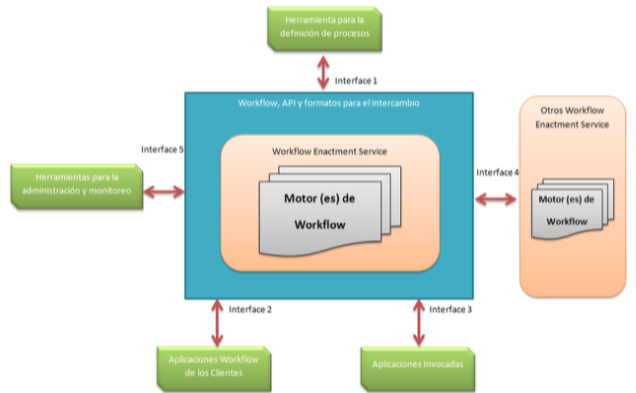
\includegraphics [scale=0.50]{imagenes/Interfaces_del_Modelo_de_Referencia.png}
	\end{center}
	\caption{Interfaces del Modelo de Referencia}
	\label{fig:Interfaces del Modelo de Referencia}
\end{figure} 

En el modelo adoptado hay una separación entre los procesos y el control de la lógica de las actividades. Esta lógica está dentro del Workflow Enactment Service. Esta separación permite la integración de las diversas herramientas con una aplicación particular. La interacción del Enactment Service con los recursos externos se da por una de las dos interfaces siguientes:

\begin{itemize}
	\item La interface de las Aplicaciones de los Clientes, a través de la cual el Motor de Workflow interactúa con el manejador de la Worklist, responsable de organizar el trabajo por intermedio de un recurso de usuario. Es responsabilidad del manejador del Worklist elegir y hacer progresar cada elemento de la lista de trabajo (Worklist).
	
	\item La interfaz de las Aplicaciones Invocadas, la cual le permite al motor de Workflow activar una herramienta para realizar una actividad particular. Esta interface podría ser basada en un servidor, es decir no existe la interacción con el usuario.
	
\end{itemize}

El Motor de Workflow (Workflow Engine) es el software que provee el control del ambiente de ejecución de una instancia de Workflow. Típicamente dicho software provee facilidades para:

\begin{itemize}
	\item Interpretación de la definición de procesos.
	
	\item Control de las instancias de los procesos: creación, activación, terminación, etc. Navegación entre actividades.
	
	\item Soporte de interacción con el usuario.
	
	\item Pasaje de datos al usuario o a aplicaciones.
	
	\item Invocación de aplicaciones externas.
\end{itemize}

Por otra parte, las WAPI pueden ser vistas como un conjunto de llamadas API (Application Programming Interface) y funciones de intercambio de datos soportadas por el Workflow Enactment Service. Las APIs son un conjunto de llamadas a funciones de software que permiten a las aplicaciones acceder a funciones de un programa. Las WAPI permiten la interacción del Workflow Enactment Service con otros recursos y aplicaciones.

\section{Web Service}
\label{Web Service}

El término Web Service se utiliza muy a menudo hoy en día, aunque no siempre con el mismo significado. Los conceptos y tecnologías subyacentes de los WS's son en gran medida independientes de la forma en que puedan ser interpretadas. Las definiciones existentes para el concepto de WS, van desde la muy genérica y con todo incluido a la muy específica y restrictiva.\\

Entonces, se puede comenzar por definir a un WS como un estándar de comunicación entre procesos y/o componentes, diseñado para ser multiplataforma y multilenguaje, es decir, no importa en qué lenguaje esté programado un WS como ser Visual Basic, C\# o Java, o en qué plataforma esté corriendo, ya sea Windows, UNIX o Linux éstos serán accesibles y utilizables por otras aplicaciones desarrolladas en otras plataformas o lenguajes de programación. Es decir, diversas aplicaciones de software desarrolladas en lenguajes de programación diferentes, y ejecutadas sobre cualquier plataforma, pueden utilizar los WS's para intercambiar datos tanto en redes locales como en Internet. Esta interoperabilidad se consigue mediante la adopción de estándares abiertos. Las organizaciones, esencialmente la W3C, son los comités responsables que se encargan de la arquitectura y la reglamentación de los WS's.\\

Precisamente la W3C define a los WS's como ``Aplicaciones de software identificadas mediante una URI (Uniform Resource Identifier), cuyas interfaces (y uso) son capaces de ser definidas, descritas y descubiertas mediante artefactos XML, y soportar interacciones directas con otras aplicaciones software usando mensajes basados en XML y protocolos basados en Internet''.\\

En el mundo de los WFMS, tanto los usuarios como los administradores de Workflow usualmente requieren la utilización de aplicaciones externas para desarrollar sus tareas, por ejemplo, aplicaciones que le permitan utilizar servicios de e-mail, fax, realizar la administración de sus documentos, u otras aplicaciones propias del usuario como obtener fechas, climas o cálculos matemáticos provistos desde la web.\\

Por otra parte, los WS's pueden ser agrupados según las funcionalidades que ofrecen en: de Información de negocios (pronóstico del tiempo, calendario, noticias, chequeo de crédito de una tarjeta, subastas, cotizaciones de acciones, planificación de vuelos, etc.); de Transacciones (reservas aéreas, acuerdos para rentar un auto, orden de compra, gestión de una cadena de suministro, etc.); o de Externalización de procesos de negocio (vínculos comerciales a nivel de Workflow, etc.).\\

Los WS's se describen en términos de sus operaciones y de los mensajes de entrada y salida de cada una de esas operaciones que provee. Tales definiciones se expresan en el lenguaje de marcado extensible XML (Extensible Markup Language) \cite{XML}, usando un lenguaje de descripción de WS's: WSDL (Web Service Description Language)\cite{WSDL2.0-0} \cite{WSDL2.0-1}. La noción de describir un WS independientemente de la tecnología en la cual ha sido implementado es robustamente capturada en este lenguaje. WSDL especifica claramente la ubicación del servicio junto con las operaciones que necesitan ser invocadas, los parámetros que deben pasarse, los tipos de datos de cada parámetro, y los distintos formatos de mensajes y tipos.\\ 

Así, el uso de protocolos estándares como WSDL en el contexto de los WS's es necesario sin excepciones para poder lograr la interoperabilidad en estos ambientes heterogéneos, con independencia del sistema operativo, el lenguaje de programación, etc. Otros estándares que se utilizan al hablar de WS's son:
\begin{itemize}
	
	\item \textbf{Protocolo HTTP (Hiper Text Transport Protocol) \cite{HTTP}:}
	 HTTP es la abreviatura de HyperText Transfer Protocol, HTTP es el protocolo utilizado por la World Wide Web. HTTP define cual es el formato de los mensajes, y cómo se transmiten los mismos.\\
	HTTP es un protocolo sin estado, se lo llama así  ya que cada comando se ejecuta de forma independiente, sin ningún conocimiento de los comandos que vinieron antes que él. Esta es la razón principal por la que es difícil de implementar sitios Web que reaccionan de forma inteligente a la entrada del usuario. Esta deficiencia de HTTP está siendo abordada en una serie de nuevas tecnologías, incluyendo ActiveX, Java, JavaScript y las cookies.
	
	\item \textbf{Protocolo SOAP (Simple Object Access Protocol) \cite{SOAP}: }
	SOAP (Simple Object Access Protocol) es el protocolo base de los WS's. Este protocolo está basado en XML y no se encuentra atado a ninguna plataforma o lenguaje de programación. A su vez, también es el protocolo más aceptado por la mayoría de las plataformas. 
	Si bien SOAP es un protocolo, éste no es exactamente un protocolo de comunicación entre mensajes como lo es el HTTP, por ejemplo. Básicamente, SOAP son documentos XML y necesitaremos utilizar algún otro protocolo para la transmisión de estos documentos como ser el protocolo HTTP o cualquier otro protocolo de comunicación capaz de transmitir textos. En la figura \ref{fig:Composición del protocolo SOAP} podemos ver como SOAP esa compuesto.
	



\begin{figure}[!h] 
	\begin{center}
		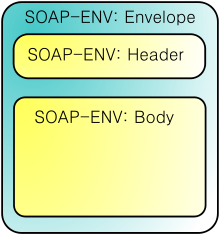
\includegraphics [scale=0.50]{imagenes/Composicion_del_protocolo_SOAP.png}
	\end{center}
	\caption{Composición del protocolo SOAP}
	\label{fig:Composición del protocolo SOAP}
\end{figure} 

	\item \textbf{UDDI (Universal Description, Discovery and Integration) \cite{UDDI}:} Se utiliza para el registro y la localización de cualquier WS. Se trata de un directorio o catálogo de WS's distribuido que permite que se listen, busquen y descubran este tipo de aplicaciones de software.
	UDDI tiene como objetivo ser accedido por los mensajes SOAP y dar paso a documentos WSDL.\\
\end{itemize}


Cada uno de estos protocolos se asocian a una capa, las cuales en conjunto, definen la infraestructura de los WS's.\\


\begin{itemize}
	\setlength{\itemindent}{.5in}
	\item[HTTP:] Corresponde La capa de transporte utilizada para el envío de la información;
	\item[SOAP:] Corresponde a la capa de mensajes.
	\item[WSDL:] Corresponde a la capa de descripción.
	\item[UDDI:] Corresponde a la capa de procesos que se encargan de la publicación, descubrimiento, composición, orquestación, desarrollo e integración de WS's. Al desaparecer los registos UDDI publicos, esta tesis plantea una solución usando una base conocida de WS's.
\end{itemize}

\subsection{El lenguaje WSDL}
\label{El lenguaje WSDL}

WSDL (Web Service Description Language) es el lenguaje de especificación utilizado para definir los WS's. Se trata de un documento XML que se utiliza para describir los mensajes SOAP y cómo estos mensajes son intercambiados. Es decir, supongamos que creamos un WS y queremos que otras aplicaciones lo utilicen, las otras aplicaciones deberán acceder a un documento WSDL en donde podrán conocer los métodos que expone nuestro WS y cómo acceder a ellos, es decir, cuáles son los nombres de los métodos y qué tipos de parámetros espera cada uno de ellos. Entonces, en este sentido, cualquier documento WSDL permite proveer información acerca de la ubicación de cierto WS y su interfaz. Así, con esta información respecto a la descripción y especificación del WS, el usuario sabrá básicamente cómo llevar a cabo la interacción con el servicio.\\

Hay que tener en cuenta que todo documento WSDL separa la descripción de un servicio en dos partes \cite{WSA}. Dentro de cada una de estas partes, se utilizan un número de constructores que promueven la reusabilidad de la descripción y permiten separarla de los detalles de diseño. Una de ellas es la interfaz abstracta, la cual describe las operaciones soportadas por el servicio, los parámetros de la operación y los tipos de datos abstractos. Esta descripción es completamente independiente de la dirección de red concreta, el protocolo de comunicación o las estructuras de datos concretas del servicio. La otra parte es la implementación concreta, la cual liga la interfaz abstracta a una dirección de red, protocolo y estructuras de datos concretas. WSDL provee toda esta información a través de elementos XML. \\

Por un lado, en la Interfaz Abstracta los dos elementos a definir son:\\

\begin{enumerate}[1.]
	\item \textbf{types:} provee la definición de los tipos de datos utilizados para describir los mensajes a intercambiar, sus operaciones los parámetros de entrada o salida de cada operación.
	
	\item \textbf{interface:} describe la secuencia de mensajes que el servicio envía o recibe.
\end{enumerate}


Y por el otro, los dos elementos a definir en la implementación concreta son:

\begin{enumerate}[1.]
	\item \textbf{binding:} define los detalles de implementación concretos del servicio.
	
	\item \textbf{service:} se usa para asociar un binding con el URL donde está realmente el servicio (endpoint).
\end{enumerate}

Entonces cualquier documento WSDL especifica tanto la definición como una descripción del WS que representa. Pero también define los dos componentes principales de estos, es decir, sus características funcionales y sus características no funcionales.  La descripción funcional se refiere a las características operacionales que definen el comportamiento general de un WS. En otras palabras, define los detalles de cómo es invocado el servicio, su ubicación, etc. Esta descripción focaliza en los detalles de la sintaxis de los mensajes y cómo configurar los protocolos de red para enviar estos mensajes. Y el otro componente, la descripción no funcional, se concentra en las características de calidad (QoS) del WS.


\subsection{Características de Calidad de los Web Services}
\label{Características de Calidad de los Web Services}

Los requerimientos de un WS no deben focalizar solamente en las propiedades funcionales del mismo, sino que también se deben concentrar en describir el ambiente en el que se desarrolla, es decir, describir las capacidades no funcionales o QoS del servicio \cite{W3C03-QoS}. Cada servicio puede ofrecer diversas opciones de características no funcionales basadas en los requerimientos técnicos como: disponibilidad, performance y escalabilidad, políticas de seguridad y privacidad, etc., todas las cuales deben ser descriptas.

Los elementos clave que se tienen en cuenta para soportar las QoS en el mundo de los WS's son:
\begin{itemize}
	\item \textbf{Rendimiento o throughput:} Número de requerimientos de WS's atendidos en un período de tiempo dado.
	
	\item \textbf{Tiempo de Respuesta:} Tiempo esperado entre que se envía un requerimiento y se recibe una respuesta.
	
	\item \textbf{Latencia:} Tiempo entre que un requerimiento de un servicio arriba y el requerimiento comienza a ser atendido.
	
	\item \textbf{Tiempo de Ejecución:} Es el tiempo que necesita un WS para procesar su secuencia de actividades.
	
	\item \textbf{Tiempo de Transacción:} Representa el tiempo que transcurre mientras el WS está completando una transacción.
	
	\item \textbf{Disponibilidad:} Probabilidad de que el WS esté disponible.
	
	\item \textbf{Fiabilidad:} Habilidad de un servicio para funcionar correcta y consistentemente y proveer la misma calidad a pesar de las fallas en la red o el sistema.
	
	\item \textbf{Precisión:} Radio de error producido por un servicio.
	
	\item \textbf{Robustez:} Grado en el cual un servicio puede funcionar correctamente en presencia de entradas inválidas, incompletas o conflictivas.
	
	\item \textbf{Reputación:} Medida de la reputación otorgada al servicio por el usuario final.
	
\end{itemize}

Tradicionalmente, las QoS se miden por el grado en el cual las aplicaciones, sistemas, redes y otros elementos de Internet soportan la disponibilidad de los servicios a un nivel requerido de performance, en todos los accesos y condiciones de descarga. En el contexto de los WS's, las QoS se pueden ver como la capacidad de ofrecer garantía sobre un conjunto de características cuantitativas, referidas específicamente a los aspectos no funcionales de los servicios. Estas características son un requerimiento necesario para entender el comportamiento subyacente del servicio de manera tal que otras aplicaciones y servicios puedan invocarlos y ejecutarlos como parte de su proceso de negocio.\\

En este trabajo se propone una forma de incorporar las QoS en los WS's a partir de la necesidad de tenerlas en cuenta a la hora de optimizar el proceso de selección del WS más adecuado. Esta incorporación ofrece importantes beneficios, tanto para los usuarios como los proveedores. A los usuarios les permite expresar sus necesidades y utilizar el WS que mejor se ajusta sus necesidades, mientras que los proveedores pueden publicar mejor las capacidades de sus servicios y lucirse con las mismas.

\section{Desarrollo de software dirigido por modelos}
\label{Desarrollo de software dirigido por modelos}

El desarrollo de software dirigido por modelos surge como respuesta a los principales problemas que actualmente tienen las compañías de desarrollo de software: por un lado, para gestionar la creciente complejidad de los sistemas que construyen y mantienen, y por otro para adaptarse a la rápida evolución de las tecnologías software.\\
En primer lugar, se usan modelos para representar tanto los sistemas como los propios artefactos del software. Cada modelo trata un aspecto del sistema, que puede ser especificado a un nivel más elevado de abstracción y de forma independiente de la tecnología utilizada. Este hecho permite que la evolución de las plataformas tecnológicas sea independiente del propio sistema, disminuyendo así sus dependencias.
En segundo lugar, se consigue también proteger gran parte de la inversión que se realiza en la informatización de un sistema, pues los modelos son los verdaderos artífices de su funcionamiento final y, por tanto, no será necesario empezar desde cero cada vez que se plantee un nuevo proyecto o se desee realizar algún tipo de mantenimiento sobre el producto.\\
En tercer lugar, en MDA los modelos constituyen la propia documentación del sistema, disminuyendo considerablemente el coste asociado y aumentando su mantenibilidad, puesto que la implementación se realiza de forma automatizada a partir de la propia documentación.

\subsection{Modelos}
\label{Modelos}

De forma sencilla podríamos definir un modelo como una abstracción simplificada de un sistema o concepto del mundo real. Un modelo de un cierto <X>  es una especificación o descripción de ese <X> desde un determinado punto de vista, expresado en un lenguaje bien definido y con un propósito determinado.\\

Según Bran Selic, uno de los fundadores del MDD y pionero en el uso de sus técnicas los modelos deberían ser:
\begin{itemize}
	\item \textbf{Adecuados:} Construidos con un propósito concreto, desde un punto de vista determinado y dirigidos a un conjunto de usuarios bien definido.
	
	\item \textbf{Abstractos:} Enfatizan los aspectos importantes para su propósito a la vez que ocultan los aspectos irrelevantes.
	
	\item \textbf{Comprensibles:} Expresados en un lenguaje fácilmente entendible para sus usuarios.
	
	\item \textbf{Precisos:} Representan fielmente al objeto o sistema modelado.
	
	\item \textbf{Predictivos:} Pueden ser usados para responder preguntas sobre el modelo e inferir conclusiones correctas.
	
	\item \textbf{Rentables:} Han de ser más fáciles y baratos de construir y estudiar que el propio sistema.
\end{itemize}

Bran Selic también señala las principales funciones que los modelos deberían tener en el ámbito de la ingeniería del software:

\begin{itemize}
	\item \textbf{Comprender el sistema}
		\begin{itemize}
			\item La estructura, el comportamiento y cualquier otra característica relevante de un sistema y su entorno desde un punto de vista dado.
			
			\item Separar adecuadamente cada uno de los aspectos, describiendolos al nivel conceptual adecuado.
		\end{itemize}
	\item \textbf{Servir de mecanismo de comunicación}
		\begin{itemize}
			\item Con los distintos tipos de stakeholder del sistema (desarrolladores, usuarios finales, personal de soporte y mantenimiento, etc.).
			
			\item Con las otras organizaciones (proveedores y clientes que necesitan comprender el sistema a la hora de interoperar con él).
		\end{itemize}	
	\item \textbf{Validar el sistema y su diseño}
		\begin{itemize}
			\item Detectar errores, omisiones y anomalías en el diseño tan pronto como sea posible (cuanto antes se detecten, menos cuesta corregirlos).
			
			\item Razonar sobre el sistema, infiriendo propiedades sobre su comportamiento (en caso de modelos ejecutables que puedan servir como prototipos).
			
			\item Poder realizar análisis formales sobre el sistema.
		\end{itemize}		
	\item \textbf{Guiar la implementación}
		\begin{itemize}
			\item Servir como ``planos'' para construir el sistema y que permitan guiar su implementación de una forma precisa y sin ambigüedades.
			
			\item Generar, de la forma más automática posible, tanto el código final como todos los artefactos necesarios para implementar, configurar y desplegar el sistema.
		\end{itemize}	
	
\end{itemize}

\subsection{Metamodelos}
\label{Metamodelos}

Un metamodelo es un modelo que especifica los conceptos de un lenguaje, las relaciones entre ellos y las reglas estructurales que restringen los posibles elementos de los modelos válidos, así como aquellas combinaciones entre elementos que respetan las reglas semánticas del dominio.
De esta forma, cada modelo se escribe en el lenguaje que define su metamodelo (su lenguaje de modelado), quedando establecida la relación entre el modelo y su metamodelo por una relación de “conformidad” (y diremos que un modelo es “conforme a” un metamodelo). Esta relación se puede observar en la figura \ref{fig:Relación modelo metamodelo}.

\begin{figure}[!h] 
	\begin{center}
		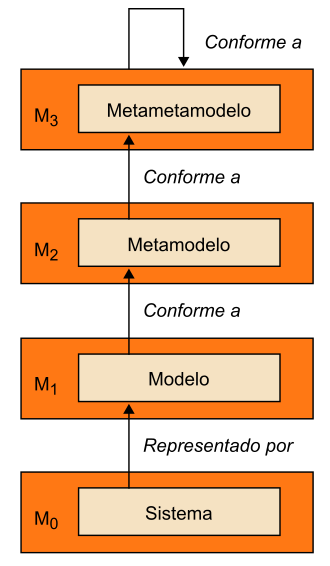
\includegraphics [scale=0.40]{imagenes/Relacion_modelo_metamodelo.png}
	\end{center}
	\caption{Relación modelo metamodelo}
	\label{fig:Relación modelo metamodelo}
\end{figure} 

\subsection{Terminología}
\label{Terminología}

La comunidad utiliza en la actualidad un conjunto de acrónimos referidos a diferentes enfoques relacionados con la ingeniería del software que usa modelos como elementos clave de sus procesos: MDD, MBE, MDA, etc. Aunque algunos de ellos ya se han mencionado en secciones anteriores, en este apartado trataremos de aclarar estos conceptos y las diferencias entre ellos.\\

MDD (model-driven development) es un paradigma de desarrollo de software que utiliza modelos para diseñar los sistemas a distintos niveles de abstracción, y secuencias de transformaciones de modelos para generar unos modelos a partir de otros hasta generar el código final de las aplicaciones en las plataformas destino \cite{3}.

MDA (model-driven architecture) es la propuesta concreta de la OMG para implementar MDD, usando las notaciones, mecanismos y herramientas estándares definidos por esa organización \cite{5}.\\

Los estándares que la OMG ofrece para realizar MDA incluyen, entre otros:

\begin{itemize}
	\item UML (unified modeling language) como lenguaje de modelado.
	\item MOF (meta-object facility) como lenguaje de metamodelado.
	\item OCL (object constraint language) como lenguaje de restricciones y consulta de modelos.
	\item QVT (query-view-transformation) como lenguaje de transformación de modelos.
	\item XMI (XML metadata interchange) como lenguaje de intercambio de información.
\end{itemize}

MDE (model-driven engineering) es un paradigma dentro de la ingeniería del software que aboga por el uso de los modelos y las transformaciones entre ellas como piezas clave para dirigir todas las actividades relacionadas con la ingeniería del software.\\

MBE (model-based engineering) es un término general que describe los enfoques dentro de la ingeniería del software que usan modelos en algunos de sus procesos o actividades.\\

BPM (business process modeling) es una rama del model-based engineering que se centra en el modelado de los procesos de negocio de una empresa u organización, de forma independiente de las plataformas y las tecnologías utilizadas.\\

Architecture-driven modernization (ADM) es una propuesta de la OMG para implementar prácticas de ingeniería inversa utilizando modelos.\\

Model driven-interoperability (MDI) es una iniciativa para implementar mecanismos de interoperabilidad entre servicios, aplicaciones y sistemas usando modelos y técnicas de MBE.\\

En la figura \ref{fig:Relacíon entre los contextos de MDE, MDD y MDA} se puede observar la relación entre los contextos de MDE, MDD, MDA.

\begin{figure}[!h] 
	\begin{center}
		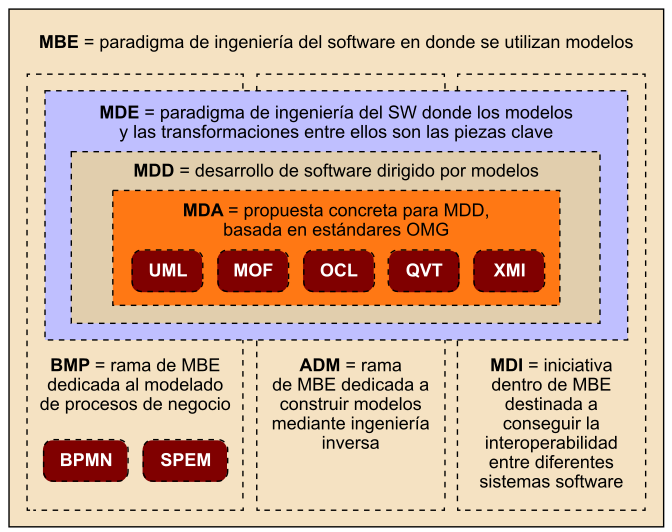
\includegraphics [scale=0.50]{imagenes/Relacion_MDE_MDD_MDA.png}
	\end{center}
	\caption{Relación entre los contextos de MDE, MDD y MDA}
	\label{fig:Relacíon entre los contextos de MDE, MDD y MDA}
\end{figure} 

\subsection{Transformaciones de modelos}
\label{Transformaciones de modelos

\subsubsection*{La necesidad de las transformaciones de modelos} 
\label{La necesidad de las transformaciones de modelos} 

Las transformaciones de modelos proporcionan los mecanismos que permiten especificar el modo de producir modelos de salida a partir de modelos de entrada.\\
El concepto de transformación en el mundo de la informática no es nuevo. De hecho, las transformaciones son algo fundamental en la ingeniería del software, pudiendo verse la computación como un proceso de transformación de datos.

Entre las aplicaciones de las transformaciones de modelo en el ámbito de MDE nos encontramos:

\begin{itemize}
	\item Generación de modelos a más bajo nivel, y finalmente código, a partir de modelos a alto nivel.
	\item Sincronización y mapping entre modelos al mismo o diferentes niveles de abstracción.
	\item Creación de vistas basadas en queries sobre un sistema.
	\item Aplicación a la ingeniería inversa para obtener modelos a más alto nivel a partir de modelos a más bajo nivel.
\end{itemize}

\subsubsection*{Conceptos básicos}
\label{Conceptos básicos}

Las transformaciones de modelos pueden verse como programas que toman un modelo (o más de uno) como entrada y retornan otro modelo (o más de uno) como salida.\\
Generalmente, una transformación de modelos está formada por un conjunto de reglas de transformación, que son consideradas como las unidades de transformación más pequeñas. Cada una de las reglas describe cómo uno o más elementos del modelo origen son transformados en uno o más elementos del modelo destino.

La figura \ref{fig:Transformación de modelo} demuestra como se lleva a cabo una transformación de modelo.

\begin{figure}[!h] 
	\begin{center}
		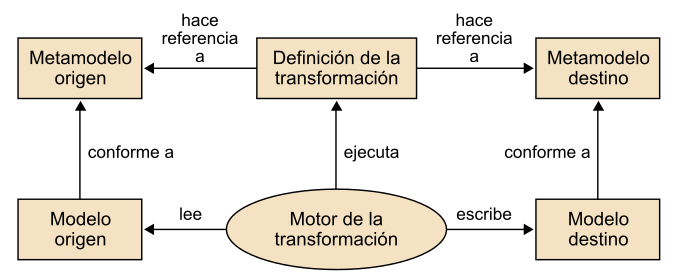
\includegraphics [scale=0.50]{imagenes/Transformacion_modelo.png}
	\end{center}
	\caption{Transformación de modelo}
	\label{fig:Transformación de modelo}
\end{figure} 

\subsubsection*{Tipos de transformaciones}
\label{Tipos de transformaciones}

En MDE se describen diferentes tipos de transformaciones entre modelos, dependiendo de varios criterios:

\begin{enumerate}[a)]
    \item Nivel de abstracción de los modelos de entrada y salida.
    \begin{itemize}
		\item Transformaciones verticales. Relacionan modelos del sistema situados en distintos niveles de abstracción y pueden aplicarse tanto en sentido descendente como en sentido ascendente, siendo estos últimos el resultado de aplicar un proceso de ingeniería inversa.
		\item Transformaciones horizontales. Relacionan los modelos que describen un sistema desde un nivel de abstracción similar. Se utilizan también para mantener la consistencia entre distintos modelos de un sistema, es decir, garantizan que la información modelada sobre una entidad en un modelo es consistente con lo que se dice sobre dicha entidad en cualquier otra especificación situada al mismo nivel de abstracción.
    \end{itemize}
    \item Tipo de lenguaje que se utiliza para especificar las reglas. Se distingue entre lenguajes declarativos, imperativos o híbridos (si permiten ambos tipos de forma combinada).
    \item Atendiendo a la direccionalidad, nos encontramos con:
    \begin{itemize}
    	\item Transformaciones unidireccionales, las reglas se ejecutan en una sola dirección.
    	\item Transformaciones bidireccionales. En estas, las transformaciones se pueden aplicar en ambas direcciones .
    \end{itemize}
    \item Dependiendo de los modelos origen y destino:
    \begin{itemize}
    	\item Transformaciones exógenas. Los metamodelos origen y destino son distintos. Es el caso más común: se tiene un modelo de entrada y se obtiene el de salida a partir de él aplicando las reglas de la transformación. 
    	\item Transformaciones endógenas. Aquí, los metamodelos origen y destino son el mismo, se trata de las llamadas transformaciones in-place: las reglas de transformación se van aplicando sobre el propio modelo de entrada, de modo que este se va transformando hasta que no se puede aplicar ninguna regla más y el modelo de entrada pasa a ser el de salida.
    \end{itemize}
    \item Atendiendo al tipo de modelo destino:
    \begin{itemize}
    	\item Transformaciones modelo a modelo (M2M), las cuales generan modelos a partir de otros modelos.
    	\item Transformaciones modelo a texto (M2T), que generan cadenas de texto a partir de modelos. Son usadas, por ejemplo, para generar código y documentos.
    	\item Transformaciones texto a modelo (T2M), que generan modelos a partir de cadenas de texto.
    \end{itemize}
\end{enumerate}

\subsubsection*{Transformaciones de modelos en MDA}
\label{Transformaciones de modelos en MDA}

Una transformación de modelos es el proceso de convertir un modelo de un sistema en otro modelo del mismo sistema. Asimismo, dícese de la especificación de dicho proceso.\\

En esencia, una transformación establece un conjunto de reglas que describen cómo un modelo expresado en un lenguaje origen puede ser transformado en un modelo en un lenguaje destino.\\

Para definir una transformación entre modelos es necesario:
\begin{enumerate}[1.]
	\item Seleccionar el tipo de transformación y el lenguaje de definición de transformaciones a utilizar 
	\item Seleccionar la herramienta que nos permita implementar los modelos y las transformaciones de forma automática.	
\end{enumerate}

\section{QVT}
\label{QVT}

QVT es la propuesta del OMG para resolver el problema de la transformación de modelos. Se trata de un estándar para la definición de transformaciones sobre modelos MOF.  La especificación de QVT depende de otros dos estándares de la OMG como son MOF y OCL.\\

El lenguaje en sí define tres diferentes lenguajes de transformación: Relations, Core y Operational.\\

En la dimensión de la interoperabilidad se encuentran aquellas características que permiten a una herramienta que cumple el estándar QVT interopere con otras herramientas.\\
Concretamente, son cuatro:

\begin{itemize}
	\item La sintaxis ejecutable se traduce en una implementación que facilite la importación o lectura, y posterior ejecución de una sintaxis concreta que describa una transformación definida en el lenguaje dado por la dimensión del lenguaje.	 	 	 	
	\item XMI ejecutable dictamina que una implementación debe facilitar la importación o lectura, y posterior ejecución de una serialización XMI de una transformación que conforma con el metamodelo de MOF del lenguaje dado por la dimensión del lenguaje. 	
	\item La sintaxis exportable establece que una implementación debe proporcionar facilidad para exportar una transformación entre modelos en la sintaxis concreta del lenguaje dado por la dimensión del lenguaje. 	 	 	
	\item XMI exportable es el nivel de interoperabilidad que debe facilitar la exportación de transformaciones entre modelos como serializaciones XMI que conformen con el metamodelo MOF del lenguaje dado por la dimensión del lenguaje.
\end{itemize}

El estándar QVT define tres abstracciones fundamentales, que se corresponden con sus siglas

\begin{itemize}
	\item \textbf{Consultas (Queries)} Una consulta es una expresión que se evalúa sobre un modelo. Los resultados de una consulta son una o varias instancias de los tipos definidos en el modelo transformado, o en el propio lenguaje de consulta. Para la realización de consultas se utilizará un lenguaje de consultas.	 	 	 	
	\item \textbf{Vistas (Views)} Una vista es un modelo obtenido en su totalidad a partir de otro modelo base. Una vista es una proyección realizada sobre un modelo, creada mediante una transformación. Una vista puede verse como el resultado de una consulta sobre un modelo, ofreciendo como resultado un punto de vista de éste, restringiéndolo de acuerdo a alguna condición impuesta.	
	\item \textbf{Transformaciones (Transformations)} Una transformación genera un modelo a partir de otro modelo de origen. Ambos modelos podrán ser dependientes o independientes, según exista o no una relación que mantenga ambos sincronizados una vez se produzca la transformación. Las vistas son un tipo específico de transformación. Las relaciones especifican las transformaciones y las correspondencias (mappings) las implementan. Son especificaciones que toman como entrada uno o varios modelos, y lo relacionan de manera que cumplan las condiciones de la transformación, o crean uno nuevo a partir de los modelos de entrada. Si se modifica una vista, la correspondiente transformación debe ser bidireccional para reflejar los cambios en el modelo fuente. Las transformaciones se definirán utilizando un lenguaje de transformación. El lenguaje de transformación debe servir para generar vistas de un metamodelo, debe ser capaz de expresar toda la información necesaria para generar automáticamente la transformación de un modelo origen a uno destino, y debe además soportar cambios incrementales en un modelo origen que se ven reflejados en el modelo destino.
\end{itemize}

De estas abstracciones se desprenden por lo tanto dos lenguajes, de consulta y de transformación, a los que se impuso como requisito que estuvieran definidos como metamodelos MOF 2.0. Un último requisito fundamental de la propuesta QVT es relativo a los modelos manipulados: todos los modelos manipulados por los mecanismos de transformación serán además instancias de metamodelos MOF 2.0.

\subsection{Arquitectura QVT}
\label{Arquitectura QVT}

La especificación de transformaciones se propone una solución de naturaleza híbrida declarativa e imperativa.\\

La parte declarativa de esta especificación está estructurada en una arquitectura de dos capas:

\begin{itemize}
	\item Un metamodelo Relations define un lenguaje declarativo para expresar relaciones entre modelos MOF. Este lenguaje soporta reconocimiento de patrones, la creación de plantillas de objetos y la creación implícita de las trazas necesarias para registrar los cambios que se producen cuando se transforman modelos.	
	\item Un metamodelo Core y un lenguaje declarativo de menor nivel de abstracción que Relations pero con la misma potencia, definido usando extensiones mínimas de EMOF y OCL. La especificación de QVT define las reglas que permiten mapear la semántica de Relations a la de Core, y dichas reglas las define en base a transformaciones descritas utilizando a su vez Core. En este lenguaje, los objetos de traza deben definirse explícitamente y sólo soporta reconocimiento de patrones sobre un conjunto plano de variables, no sobre objetos complejos como en Relations.
\end{itemize}

\subsection{Escenarios de ejecución}
\label{Escenarios de ejecución}

La semántica del lenguaje Core y el lenguaje Relaciones debe tener en cuenta los siguientes escenarios de ejecución:
\begin{itemize}
	\item Entradas a sólo transformaciones para verificar que los modelos se relacionan de una manera específica.	
	\item Transformaciones de una sola dirección.	
	\item Transformaciones bidireccionales.
	\item La capacidad de establecer relaciones entre los modelos preexistentes.
	\item Actualizaciones incrementales cuando un modelo relacionado se cambia después de una ejecución inicial.
	\item La capacidad de crear y eliminar objetos y valores, al mismo tiempo ser capaz de especificar los objetos y los valores que no pueden ser modificados.
\end{itemize}

\subsection{Metamodelos MOF}
\label{Metamodelos MOF}

Esta especificación define tres paquetes principales, uno para cada uno de los idiomas definidos: QVTCore, QVTRelation , y QVTOperational . El paquete QVTBase define la estructura común para las transformaciones . Además, el paquete QVTRelation utiliza expresiones de plantilla de patrones definidos en el paquete QVTTemplateExp.\\
QVTOperational extiende QVTRelation, ya que utiliza el mismo marco de rastros definidos en ese paquete. Utiliza expresiones imperativas definidas en el paquete ImperativeOCL.\\
Todos QVT depende del paquete EssentialOCL de OCL 2,0, y todos los paquetes de idioma dependen de EMOF.

\subsection{Lenguaje Relation}
\label{Lenguaje Relation}


El lenguaje Relations ofrece una aproximación declarativa para la especificación de transformaciones. Dado un par de modelos candidatos para la transformación, que deberán ser instancias de metamodelos MOF, ésta quedará definida como un conjunto de restricciones que los elementos de los modelos deben satisfacer.\\
Estas restricciones constituyen el concepto de relación del lenguaje Relations: se definen mediante dos o más dominios y mediante una pareja de predicados when (cuándo) y where (cómo). Los dominios especifican, mediante un patrón, qué elementos de los modelos candidatos participarán en la transformación. Por su parte, la cláusula when especifica la relaciones que determinan cuándo la relación indicada debe sostenerse; y la cláusula where especifica la condición que deben satisfacer todos los elementos de modelos que participan en la relación.\\

En el lenguaje Relations, una transformación entre modelos candidatos se especifica como un conjunto de relaciones que han de tener lugar para llevar a cabo la transformación.\\
Un modelo candidato es cualquier modelo que conforme a un tipo de modelo o metamodelo, que es una especificación de los diferentes tipos que pueden tener los elementos del modelo que lo conforma. Los modelos candidatos tienen un nombre y los tipos de los elementos que pueden contener, los cuales quedan restringidos al paquete al que se hace referencia en la declaración del modelo candidato. Por ejemplo:\\

\letraEcore{transformation uml2Rdbms (uml : SimpleUML, rdbms : SimpleRDBMS)}\\

En esta declaración de transformación llamada \letraEcore{uml2Rdbms}, hay dos modelos candidatos: \letraEcore{uml} y \letraEcore{rdbms}. El modelo \letraEcore{uml} se declara referenciando el paquete \letraEcore{SimpleUML} como su metamodelo, y el modelo \letraEcore{rdbms} hace lo propio con el paquete \letraEcore{SimpleRDBMS}. Una \letraEcore{transformation} puede invocarse tanto para comprobar la consistencia de dos modelos como para transformar un modelo en otro.\\
\chapter{Método para evaluar la calidad de servicio de Web Services}
\label{Método para evaluar la calidad de servicio de Web Services}

El número cada vez mayor de Web Service (WS) disponibles dentro de una organización y en la web, plantea un problema de la búsqueda de ellos, y destaca la importante necesidad de encontrar un mejor WS que cumpla con ciertos requisitos del solicitante. Por esta razón, los requisitos de un WS no deben centrarse solamente en sus propiedades funcionales, sino también en la descripción del entorno en el que se desarrolla, es decir, la descripción de características de calidad (QoS). Cada servicio puede ofrecer varias opciones para QoS basados en normas técnicas, tales como la disponibilidad, el rendimiento y la escalabilidad, las políticas de seguridad y privacidad, etc., todos los cuales deben ser descritos y analizados. En este punto, es de vital importancia contar con un procedimiento para evaluar la calidad de la WS. Este procedimiento proporcionará una herramienta para estimar la calidad de los WS de una manera específica. \\
En consecuencia de lo expuesto hasta ahora, este capítulo propone un procedimiento para medir la calidad de la WS, desarrollado en base a la publicación \cite{QoS-WS-invoked}.\\

\section{Características de calidad de Web Services}
\label{Características de calidad de Web Services}

La descripción de un WS tiene dos componentes principales: sus características funcionales y no funcionales. La descripción funcional, como mencionamos anteriormente, es una descripción sintáctica que se centra en los aspectos funcionales, detallando las características operativas que definen el comportamiento general de un WS. Un requisito importante para las aplicaciones basadas en SOA es operar de forma fiable y ofrecer un servicio consistente a una variedad de niveles. Por lo tanto, los requisitos de un WS no deben centrarse sólo en sus propiedades funcionales, sino también en la descripción del entorno que lo aloja, es decir, las capacidades no funcionales o QoS del servicio. Cada servicio puede ofrecer varias opciones para características no funcionales en base a los requisitos técnicos que resultan de la demanda de disponibilidad, el rendimiento, la escalabilidad, las políticas de seguridad, privacidad, etc., todo lo cual debe ser descrito.\\
La descripción no funcional define la QoS del servicio, obligan a el solicitante a especificar, en tiempo de ejecución, los atributos de calidad que pueden influir en la elección de un WS ofrecido por un proveedor.

\section{Marco general de selección de WS de un WFMS}
\label{Marco general de selección de WS de un WFMS}

La descripción y la automatización de procesos de negocio se realizan a través de los Workflow Management System (WFMS). El modelo de referencia del workflow, desarrollado por la WfMC define un marco genérico para la construcción de WFMS, lo que permite la interoperabilidad entre ellos y otras aplicaciones implicadas. Este modelo define una interfaz para la invocación de aplicaciones externas. \\
Para seleccionar la aplicación más adecuada entre varias semánticamente correctas que se comportan de la misma manera pero que tienen diferentes descripciones sintácticas y QoS, se propone optimizar la selección al incorporar las QoS. El esquema propuesto para la invocación de WS presenta inicialmente una muestra de los WS disponibles en una base de datos conocida, el WS requerido en la invocación de aplicaciones externas que corresponden al motor del workflow y la selección WS que eventualmente será invocado. En el método propuesto se consideran dos elementos importantes para que el proceso contraste entre los servicios ofrecidos y la aplicación requerida:

\begin{itemize}
	\item Antecedentes de ejecuciones: el método propone realizar la invocación de WS, supervisar sus atributos y registros de calidad en el historial de ejecuciones.
	\item Las características del método: el método tiene un registro de características cualitativas para invocar una aplicación.
\end{itemize}

En la realización del proceso de contraste con el nivel de calidad de servicio, el método propuesto considera:

\begin{itemize}
	\item Antes de invocar cualquier WS se analizan las características durante el proceso de verificación. Se aplica métricas para evaluar los atributos de calidad.
	\item Si el WS se ha invocado anteriormente, el método propuesto busca en la historia de las ejecuciones y observa la información almacenada del mismo.
\end{itemize}

Cuando el proceso de contraste se realiza en el nivel de calidad de servicio, es un filtro de la lista preliminar de WS candidatos y obtiene el que mejor cumpla con los requisitos del solicitante.
En el esquema propuesto, el componente principal es el descubrimiento de servicios basado en los requisitos funcionales y QoS especificados por el usuario y los requisitos por el propio motor. De este modo, el motor proporciona un ranking de WS disponible y elige el más adecuado. También es responsable de la recolección y procesamiento de información de los WS disponibles en la base de datos y mantenerla actualizada a medida que se realizan las llamadas.

\section{Método para seleccionar un WS teniendo en cuenta su calidad de servicio}
\label{Método para seleccionar un WS teniendo en cuenta su calidad de servicio}

Hemos propuesto un método de medición para obtener un valor cuantitativo de cada servicio que permite la comparación entre ellos.


En primer lugar, se define una unidad de medida que depende de la característica que está siendo evaluado. Aquí hemos considerado:
\begin{itemize}
	\item Unidad de tiempo: le asigna un valor en milisegundos, segundos, minutos u horas, dependiendo de las características que se evalúa.
	\item Porcentaje: asignado un valor numérico entre 0 y 100, que se toma de una muestra representativa, y que depende de la propiedad que está siendo evaluada.
\end{itemize}
El tiempo de respuesta (TR) se evalúan teniendo en cuenta la unidad de medida de tiempo en milisegundos. La disponibilidad (D) y la reputación (R) se mide en porcentaje.\\

La función de prioridad (Fp) asignado a cada WS un peso se define por:\\

\emph{Fp = D + R - TR}\\

Es fácil visualizar que mientras más grande sea la disponibilidad y la reputación y menor sea el tiempo de respuesta mayor será el peso de clasificación del WS.\\

La evaluación del sistema se puede hacer usando técnicas cualitativas o cuantitativas. Las técnicas cualitativas se basan en el análisis de una lista de características ,ventajas y desventajas, que se comparan de manera intuitiva para generar una clasificación final de los sistemas propuestos.\\
 
Los métodos cuantitativos dan indicadores cuantitativos generales que serán utilizadas para encontrar y justificar la decisión óptima.
Generalmente, los métodos cuantitativos basados en técnicas de puntuación tienen dos indicadores para cada sistema, estas son una puntuación de preferencia global y un indicador de costo total. Esta propuesta no tiene en cuenta el costo.\\
Los WS se utilizan mucho hoy en día, y con el creciente número de servicios disponibles que realizan la misma función, es necesario decidir qué servicio será elegido para completar una tarea dada. El objetivo es elegir el servicio más adecuado que satisfaga tanto los requisitos funcionales y no funcionales.\\
La automatización de los procesos de negocio se considera como parte de un interés principal de las organizaciones para el crecimiento, el desarrollo y la competitividad. El uso de programas como parte de Interfaz de las Aplicaciones Invocadas de los WFMS ofrece beneficios importantes, tales como la distribución transparente de las aplicaciones fuera del workflow, permitiendo que el motor invoque la aplicación sin conocer su ubicación exacta, con el importante beneficio que puede cambiar su ubicación en la red sin que suponga un cambio en su invocación. Además, los sistemas de gestión deben invocar la aplicación de workflow que es más adecuada a sus necesidades, y esto requiere la especificación de algunas restricciones que se escribirán en la memoria no funcional de una solicitud de WS.\\
Existe una clara necesidad de desarrollar mecanismos rápidos y eficaces que se pueden utilizar para la selección dinámica de los servicios a partir de un conjunto de proveedores de servicios. En este capítulo se presentó un método cuantitativo para medir las características no funcionales de los servicios que proporcionan la misma funcionalidad. El método puede medir y luego comparar las puntuaciones obtenidas por todos los servicios candidatos y seleccionar el WS que mejor se adapte a las necesidades del solicitante. En este capítulo, el método presentado se aplica a la selección dinámica de WS que puede ser utilizado por un motor de workflow cuando se requiere aplicaciones externas para llevar a cabo los procesos de negocio. 

\chapter{Mecanismo de selección de Web Services}
\label{Mecanismo de selección de Web Services}

Para permitir que la aplicación desarrollada (QVTWSinvoker) pueda seleccionar el Web Services(WS) más conveniente entre varios que semánticamente se comportan igual, se propone optimizar esta selección de servicios usando transformaciones de modelo definidos incorporando a la selección automática los atributos de calidad descriptos en el capítulo. Las transformaciones de modelo QVT permiten proveer una especificación semántica más precisa de un WS y establecer una correspondencia entre los requerimientos del usuario y los WS's disponibles, lo cual facilita su descubrimiento automático en tiempo de ejecución. 

\section{Preselección automática de WS's mediante tranfomaciones de modelo QVT}
\label{Preselección automática de WS's mediante tranfomaciones de modelo QVT}

Las figuras \ref{fig:Transformación Wsdl Ecore Request} y \ref{fig:Comparación Ecore Wsdl - Ecore Request}. presentan un esquema de la propuesta de invocación de WS's con QVT. En la misma se visualizan los WS's conocidos mediante la base de datos en formato wsdl y las carecteristicas solicitadas a través de los requisitos del usuario en un ecore request, la correspondencia realizada por el software, y la preselección de los WS's a los cuales se les evaluará su calidad. Aquí se puede observar el comportamiento interno del software a la hora de preseleccionar una aplicación externa, en particular, cómo hace el programa para preelegir la aplicación, valiéndose de los WS's disponibles en la base de datos. En el esquema propuesto, el componente principal es QVTWSinvoker, quien actúa como una agente de descubrimiento y preselección de servicios, basándose en los requerimientos funcionales por el usuario. Así, QVTWSinvoker  realiza una serie de transformaciones de los WS's disponibles y elige el más adecuado. 

Para realizar la correspondencia y preselección QVTWSinvoker trabaja en tres etapas.
\begin{itemize}
	\item En la primer etapa se transforman todos los WSDL conocidos a archivos XMI, cuyo contenido contiene la representación del modelo Ecore del WSDL, a través de una transformación T2M.
	
	\item En la segunda etapa se transforman todos los archivos XMI (WSDL Ecores) resultantes de la primer etapa a su respectiva representación Ecore del modelo de los requerimientos del usuario (Request Ecore) a través de una transformación M2M.
	
	\item En la tercer etapa establece la correspondencia teniendo en cuenta los requisitos del solicitante y los WS's transformados. Al solicitante, se le pide el tipo de aplicación, el nombre del método y los parámetros. Como resultado de la correspondencia, QVTWSinvoker obtiene una lista de los WS's precandidatos a invocarse
\end{itemize}

\begin{figure}[!h] 
	\begin{center}
		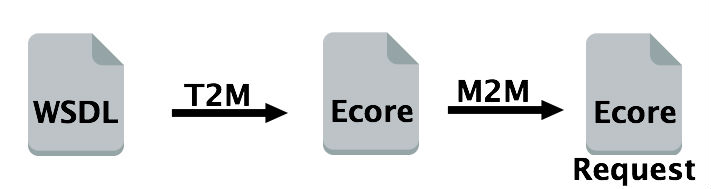
\includegraphics [scale=0.50]{imagenes/Transformacion_Wsdl_Ecore_Request.jpg}
	\end{center}
	\caption{Transformación Wsdl Ecore Request.}
	\label{fig:Transformación Wsdl Ecore Request}
\end{figure} 

\begin{figure}[!h] 
	\begin{center}
		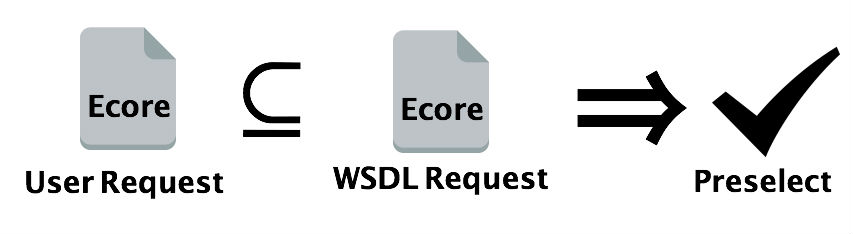
\includegraphics [scale=0.45]{imagenes/Comparacion_Ecore_Wsdl.jpg}
	\end{center}
	\caption{Comparación Ecore Wsdl - Ecore Request.}
	\label{fig:Comparación Ecore Wsdl - Ecore Request}
\end{figure} 

\section{Modelos del solicitante y los proveedores de WS's}
\label{Modelos del solicitante y los proveedores de WS's}

Para la transformación de modelos se debió utilizar dos modelos Ecore, uno que representa la solicitud del cliente, y el segundo representa un WS con formato WSDL.

\subsection{Modelo de solicitud de usuario}
\label{Modelo de solicitud de usuario}

Este modelo ecore se utiliza para representar una petición  de un cliente. La representación en diagrama de UML se realiza mediante el plugin Ecore Diagram Editor SDK.\\

Un RequestModel tendrá asociado o no, uno o varios métodos, cada método deberá tener un nombre y posiblemente una descripción de lo que hace el método. El sistema buscará precandidatos en base al nombre del método el cual contendrá parámetros de entrada y salida, el cliente solo tendrá acceso a los parámetros de entrada. Cada parámetro deberá tener un tipo predefinido de Java y un nombre (ver figura \ref{fig:Diagrama UML de RequestModel}).\\

Para obtener este modelo, se realiza una transformación T2M (ver código \ref{code:Transformación T2M RequestModel}), en donde se carga y genera un modelo RequestModel con los datos obtenidos desde una interfaz gráfica en la cual el usuario carga los requerimientos que desea.\\

\lstinputlisting[language=Java, firstline=103, lastline=161, caption={Transformación T2M RequestModel},label={code:Transformación T2M RequestModel}]{../QVTWSInvoker/src/tesis/controllers/InvokerController.java}





\begin{figure}[!h] 
	\begin{center}
		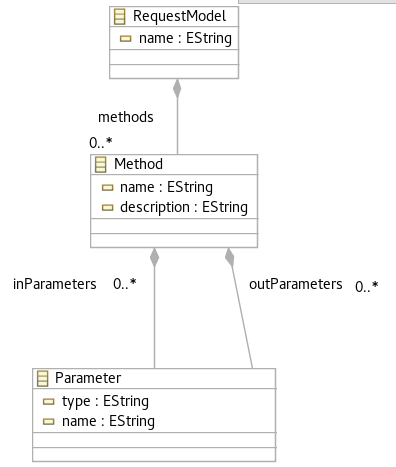
\includegraphics [scale=0.45]{imagenes/Diagrama_UML_RequestModel.png}
	\end{center}
	\caption{Diagrama UML de RequestModel.}
	\label{fig:Diagrama UML de RequestModel}
\end{figure} 

Por otro lado un WS se representa mediante un modelo ecore WSDL, al cual se le ha agregando una descripción en las operaciones. \\

Para obtener un modelo ecore de este tipo, se realiza una transformación T2M, en donde el archivo con extensión .wsdl debe estar escrito en una versión de SOAP 1.1 o 1.2. 

\section{Estructura del proyecto de transformación}
\label{Estructura del proyecto de transformación}

El proyecto consiste de 3 módulos:
\begin{itemize}
	\item \textbf{T2MWsdl:} Este módulo realiza la transformación de texto a modelo de un wsdl.
	\item \textbf{Comparsion:} Este módulo contiene la comparación de modelos, ambos modelos deben ser RequestModel.
	\item \textbf{Transformation:} Este módulo ejecuta en la transformación M2M de un wsdl, invocando la transformación QVTO definida.
\end{itemize}

Para la representación de los dos modelos ecore en Java,  se utilizó el plugin de eclipse EMF (Eclipse Modeling Framework SDK) que autogenera el código Java para la representación del mismo.\\
Esta representación en java consiste en 3 paquetes:

\begin{itemize}
	\item \textbf{utils:} Tiene clases auxiliares.
	\item \textbf{Impl:} Contiene la implementación de las interfaces.
	\item \textbf{Interface:} Comprende la representación de cada objeto del modelo ecore.
\end{itemize}

\section{Funcionamiento de la transformación}

El método consiste en 3 fases fundamentales, la primer etapa se encarga de la transformación de un wsdl en texto plano a un modelo ecore del mismo, la segunda etapa realiza la conversión M2M del modelo generado en la primer etapa a su respectiva representación en RequestModel, por último, la tercer etapa consiste en la comparación de 2 modelos RequestModel, el generado en la segunda etapa y la solicitud del usuario. Esta etapa deberá decidir si wsdl satisface la solicitud del usuario en base los criterios de comparación descritos al inicio del capítulo. \\


\textbf{Etapa 1: Transformación T2M wsdl}\\

Esta etapa realiza una transformación del wsdl en texto plano a una representación del mismo en ecore. Para ello, debemos conocer la ubicación de algún WS, por ejemplo : \url{www.dominio\_del\_web\_service.com/servicio\_web.asmx?WSDL}\\

El sistema, con el soporte de la API soa\_model\_distribution, realiza un análisis gramatical del WS para hacer más eficiente su uso (ver código \ref{code:Transformación T2M RequestModel}), luego se procede a obtener los binding del WS que se encuentran definidos para trabajar con SOAP 1.1 y 1.2 y de cada binding se consiguen los PortType.

\lstinputlisting[language=Java, firstline=40, lastline=69,caption={Análisis gramatical del WS.},label={code:Análisis gramatical del WS}]{../proyecto_eclipse/src/t2m/T2Mwsdl.java}

Luego a cada PortType, se le extraen las operaciones y se las analizan para obtener operaciones definidas en el modelo ecore (ver código \ref{code:Extraccion de operaciones de PortType}).

\lstinputlisting[language=Java, firstline=118, lastline=133,caption={Extracción de operaciones de PortType.},label={code:Extraccion de operaciones de PortType}]{../proyecto_eclipse/src/t2m/T2Mwsdl.java}

Según la definición de un wsdl, cada operación consta de mensajes de entrada y mensajes de salida. Los mensajes pueden estar definidos con tipos simples, o utilizar tipos embebidos, a su vez, un tipo embebido puede contener otros tipos embebidos, por lo tanto se emplea la recursividad para “desenvolver” los parámetros y generar parámetros de tipos simples (ver código \ref{code:Parser de messages} y \ref{code:Analisis y parser de tipos embebidos}).

\lstinputlisting[language=Java, firstline=194, lastline=218,caption={Parser de messages.},label={code:Parser de messages}]{../proyecto_eclipse/src/t2m/T2Mwsdl.java}

\lstinputlisting[language=Java, firstline=220, lastline=247,caption={Análisis y parser de tipos embebidos.},label={code:Analisis y parser de tipos embebidos}]{../proyecto_eclipse/src/t2m/T2Mwsdl.java}

Al terminar todo el análisis, se obtiene el mismo wsdl pero cargado en un modelo ecore, el cual es exportado y almacenado en disco con una extensión .xmi para luego ser utilizado en la etapa 2.\\

\textbf{Etapa 2: Transformación QVTO}\\

Esta etapa es la encargada de llevar a cabo la transformación QVTO del modelo ecore wsdl en a un modelo ecore RequestModel. El sistema comienza tomando la ruta al archivo que se generó en la etapa anterior, y una ruta de salida donde se almacenará el RequestModel.(ver código \ref{code:Invocación de la transformación qvto})

\lstinputlisting[language=Java, firstline=25, lastline=65,caption={Invocación de la transformación QVTO},label={code:Invocación de la transformación qvto}]{../proyecto_eclipse/src/t2m/Transformation.java}

Este método, como se puede visualizar, invoca la transformación qvto almacenada en otra carpeta dentro del mismo proyecto. La transformación toma como archivo de entrada un modelo wsdl y retorna un modelo RequestModel (ver código \ref{code:Perfiles y modelos de la transformación}).


\lstinputlisting[ firstline=1, lastline=5,caption={Perfiles y modelos de la transformación},label={code:Perfiles y modelos de la transformación.}]{../proyecto_eclipse/transforms/wsdlToRequest.qvto}

La transformación comienza buscando el objeto Definition en el wsdl, este es el que contiene toda la información necesaria para poder llevar adelante la transformación. Una vez obtenido la Definition, le aplica una transformación model2Request, obteniendo de esta forma el modelo RequestModel (ver código \ref{code:Inicio de la transformación QVT}).

\lstinputlisting[ firstline=7, lastline=20,caption={Inicio de la transformación QVT.},label={code:Inicio de la transformación QVT}]{../proyecto_eclipse/transforms/wsdlToRequest.qvto}

Una vez dentro de Definition, el paso siguiente es,  asignar al RequestModel el nombre de Definition, y obtener los portType, que contiene la definición de los métodos, por lo tanto se le aplica una transformación \texttt{portType2Methods}, la cual retorna un conjunto de \texttt{Methods} pertenecientes al modelo RequestModel (ver código \ref{code:Transformación PortType a Method}).

\lstinputlisting[ firstline=22, lastline=36,caption={Transformación PortType a Method},label={code:Transformación PortType a Method}]{../proyecto_eclipse/transforms/wsdlToRequest.qvto}

De esta manera, se continúa transformando hasta llegar a la parte más “interna”, donde se encuentran los métodos.  Al finalizar la transformación, se consigue la representación del wsdl en RequestModel, el cual, únicamente contiene la información necesaria, es decir, los métodos con sus respectivos parámetros de entrada y salida.\\

\textbf{Etapa 2: Comparación}\\

Una vez obtenido el/los wsdl representado/s en un modelo ecore RequestModel la petición del usuario representado de la misma forma, se comparan para decidir si la petición está o no incluida en el wsdl, y en caso de estar incluido, se considerará que el wsdl resuelve la petición del usuario.

Esta comparación se realiza con comparaciones de modelos desde Java, tomando un wsdl y la petición del usuario y comparándolos por nombres de métodos, si los nombres coinciden, se continúa analizando la cantidad de parámetros de entrada que posee cada método, en caso de ser la misma, se analizan los tipos (ver código \ref{code:Transformación de un método}).

\lstinputlisting[language=Java, firstline=15, lastline=62,caption={Transformación de un método.},label={code:Transformación de un método}]{../proyecto_eclipse/src/t2m/Comparsion.java}

La transformación QVTO es no determinista a la hora de aplicar una transformación y no respeta el orden de los parámetros, por lo tanto se procedió a ordernar los parámetros de ambos modelos de acuerdo al tipo.

Si los tipos son correctos, la comparación retorna una lista con los nombres de todos los métodos que satisfacen la petición del usuario.

\section{Análisis de la correspondencia entre los modelos generados}

Ahora, para decidir automáticamente si un WS ofrecido por un proveedor satisface la demanda del solicitante, es necesario comparar los ecore generados por dicho solicitante y proveedor. Se formaliza usando relaciones subecore. Si la precondición del solicitante es un subecore de la precondición del proveedor, entonces el proveedor provee toda la información necesaria para ejecutar el WS.

En la Figura \ref{fig:Ecores de Petición de usuario y WS 1} se puede observar que el modelo del WS 1 es un submodelo del modelo del solicitante.

\begin{figure}[!h] 
	\begin{center}
		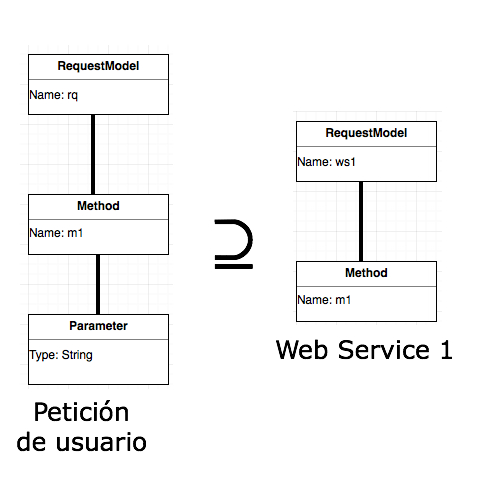
\includegraphics [scale=0.60]{imagenes/Ecores_de_Peticion_de_usuario_y_WS_1.jpg}
	\end{center}
	\caption{Ecores de Petición de usuario y WS 1.}
	\label{fig:Ecores de Petición de usuario y WS 1}
\end{figure} 

\begin{figure}[!h] 
	\begin{center}
		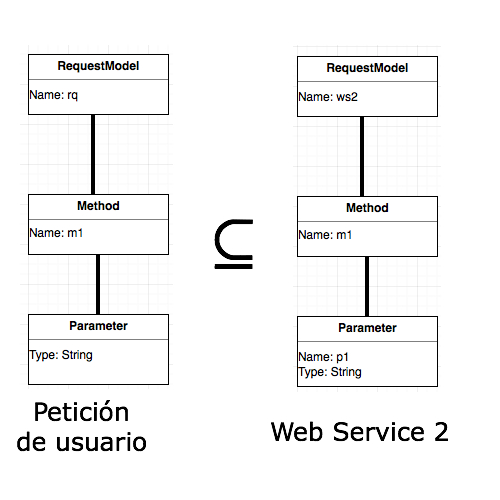
\includegraphics [scale=0.60]{imagenes/Ecores_de_Peticion_de_usuario_y_WS_2.jpg}
	\end{center}
	\caption{Ecores de Petición de usuario y WS 2.}
	\label{fig:Ecores de Petición de usuario y WS 2}
\end{figure} 

Análogamente, en la Figura \ref{fig:Ecores de Petición de usuario y WS 2} se puede observar que la peticion de usuario es un submodelo del WS 2. Por lo tanto, el proveedor 2 ofrece un WS's que son compatibles con los requerimientos del solicitante, es decir, el proveedor 2 provee toda la información necesaria para ejecutar el WS.
\chapter{Caso de estudio: QVTWSInvoker}
\label{Caso de estudio: QVTWSInvoker}

En este capítulo se presenta un caso de estudio que plantea el uso de Web Services (WS) seleccionados automáticamente en la invocación de aplicaciones externas desde un Workflow, a través de su aplicación en el marco de las tareas involucradas en el proceso de desarrollo de software denominado QVTWSInvoker.


\section{Descripción general de la herramienta}

En virtud de lograr el cumplimiento de los objetivos enunciados en la sección 1.2 una gran cantidad de factores han sido tenidos en cuenta para finalmente llegar a una solución acorde a las expectativas.\\
QVTWSInvoker utiliza una plantilla genéricas de entrada. Consiste de un conjunto de parámetros que son los encargados de transportar los requerimientos del usuario a la herramienta. Y dado que este usuario será en reiteradas ocasiones un WFMS, el conjunto de parámetros ha sido planteado simple y estándar. Esta plantilla está formada por los siguientes atributos: tipo de WS, nombres y descripción de la operación a ejecutar con sus respectivos parámetros (valores para los cuales se deseen obtener los resultados correspondientes). Esta parametrización le posibilitará a la herramienta acceder de manera estándar a los requerimientos del sistema siempre de una misma forma, para luego comenzar el proceso de búsqueda con los criterios y filtros correspondientes.\\
La salida de la herramienta se imprime en un texto simple. Luego de la salida se le pide al usuario que especifique si está satisfecho con el resultado del WS.\\
Es importante destacar, que la herramienta provee al usuario las diferentes alternativas que desee en cuanto al tipo de WS y además, le da la posibilidad de proveer información para actualizar las características de calidad (QoS) que implementa dicho WS. 

\section{Proceso de selección de WS's}

El proceso de selección de WS's con sus respectivas ejecuciones, consiste en la transformación de los requerimientos del usuario en una instancia de salida. Este proceso lo realiza QVTWSinvoker implementando los mecanismos descritos en los capítulos \ref{Mecanismo de selección de Web Services} y \ref{Caso de estudio: QVTWSInvoker} que se describe en los siguientes puntos:\\

\textbf{Fase 1: Obtención de Parámetros}\\

En esta fase la herramienta obtiene desde la plantilla de entrada los parámetros, los números del mensaje de entrada se corresponden a estos parámetros. Ellos significan: 1 = tipo del WS; 2 = nombre de las operaciones; 3 = descripción ; 4 = cantidad y tipo de los parámetros; (Ver figura \ref{fig:Plantilla de entrada de solicitud de usuario})\\

\begin{figure}[!h] 
	\begin{center}
		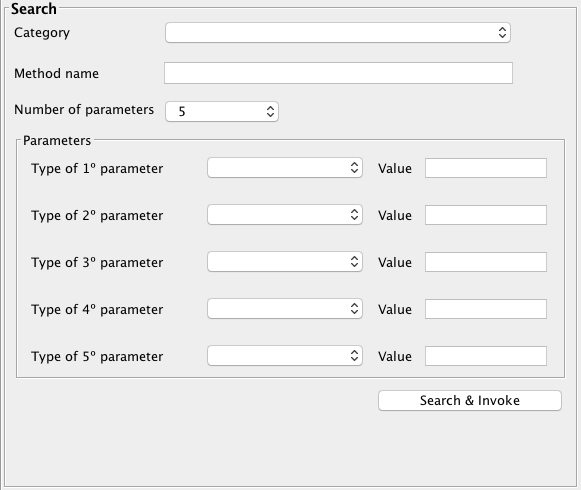
\includegraphics [scale=0.60]{imagenes/Plantilla_de_entrada_de_solicitud_de_usuario.png}
	\end{center}
	\caption{Plantilla de entrada de solicitud de usuario}
	\label{fig:Plantilla de entrada de solicitud de usuario}
\end{figure} 

\textbf{Fase 2: Obtención de WS's de la base de datos}\\

La base de datos contiene los WS's conocidos por la herramienta. Se compone de la información los WSDL y las QoS.  En esta fase la herramienta, en base al tipo ingresado por el usuario en la plantilla de entrada y las QoS , obtiene de la base de datos la lista de descripciones de los WS's ordenada por valor de ponderación de las QoS (mecanismo de calificación descrito en el capítulo \ref{Mecanismo de selección de Web Services}). 

\lstinputlisting[ firstline=113, lastline=129,caption={Método que obtiene de la base de datos la lista de descripciones},label={code:Método que obtiene de la base de datos la lista de descripciones}]{../QVTWSInvoker/src/tesis/crud/CategoryCRUD.java}

\lstinputlisting[ firstline=8, lastline=15,caption={Método comparador para ordenar la cola},label={code:Método comparador para ordenar la cola}]{../QVTWSInvoker/src/tesis/utils/WsdlComparator.java}


\textbf{Fase 3: Transformaciones y Filtro por nombre, descripción y parámetros de la operación}\\

A partir del conjunto de WS's generado en la fase previa, la herramienta procede a transformarlas siguiendo el mecanismo descripto en el cap 5 y filtrarlos teniendo en cuenta nombre, descripción y parámetros de la operación que se especificaron en la plantilla de entrada.\\	

\textbf{Fase 4. Ejecución de WS's}\\

En la ejecución de WS's se selecciona el primer WS del conjunto. Una ejecución consiste en la invocación del WS con los parámetros que el usuario pasa en la plantilla de entrada. Si el resultado de esta ejecución es exitoso, la herramienta retorna la salida cuyos datos son los obtenidos de la ejecución.\\
Una ejecución se considera exitosa cuando se muestran  los datos obtenidos de la invocación del WS. Si la ejecución no es exitosa se toma el siguiente WS y se repite esta fase.


\lstinputlisting[ firstline=215, lastline=244,caption={Invocación al mejor WS},label={code:Invocación al mejor WS}]{../QVTWSInvoker/src/tesis/controllers/InvokerController.java}


\textbf{Fase 5: Calificación del WS's}\\

Esta última fase le solicita al usuario información respecto a la calidad del servicio preguntándole si la salida ha satisfecho sus necesidades. Luego de que compute la respuesta, esta se utiliza para calcular la reputación del servicio.


\begin{figure}[!h] 
	\begin{center}
		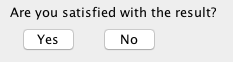
\includegraphics [scale=1.00]{imagenes/Interfaz_de_usuario_satisfecho.png}
	\end{center}
	\caption{Interfaz de usuario correspondiente a la fase 5}
	\label{fig:Interfaz de usuario correspondiente a la fase 5}
\end{figure} 


\lstinputlisting[ firstline=76, lastline=92,caption={Controlador que captura la respuesta del usuario},label={code:Controlador que captura la respuesta del usuario}]{../QVTWSInvoker/src/tesis/controllers/InvokerController.java}

\lstinputlisting[ firstline=123, lastline=148,caption={Método que edita la reputación del WS en la base de datos},label={code:Método que edita la reputación del WS en la base de datos}]{../QVTWSInvoker/src/tesis/crud/WsdlCRUD.java}

\section{Diseño de la herramienta}

\subsection{Arquitectura general}

\begin{figure}[!h] 
	\begin{center}
		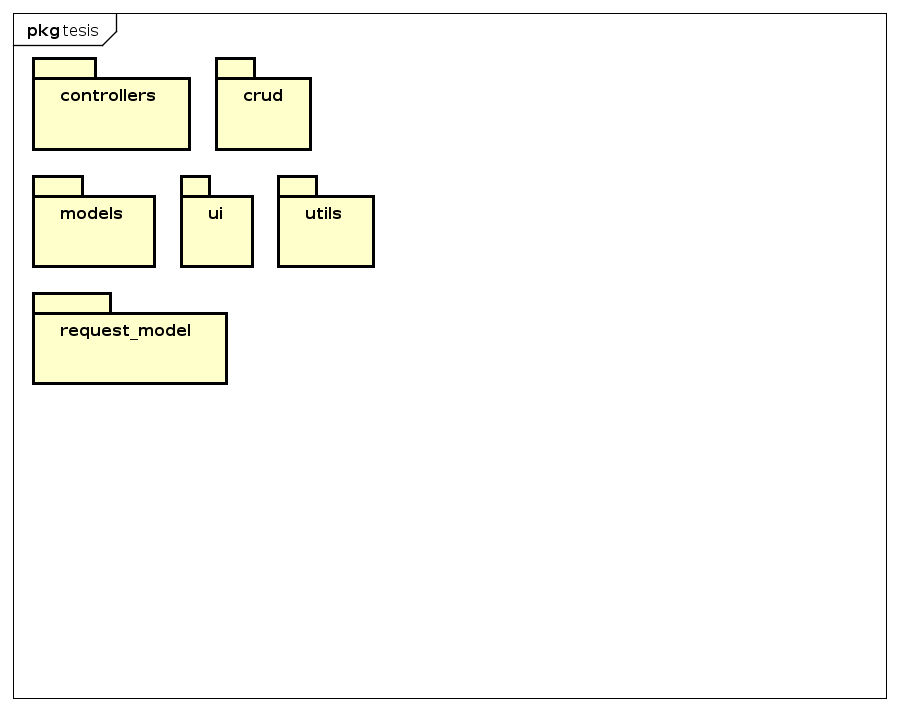
\includegraphics [scale=0.70]{imagenes/paquetes.png}
	\end{center}
	\caption{Paquetes del proyecto}
	\label{fig:Paquetes del proyecto}
\end{figure} 

La arquitectura del programa se basa en el patrón modelo–vista–controlador (MVC) \cite{MVC}, el cual separa los datos y la lógica de negocio de una aplicación de la interfaz de usuario y el módulo encargado de gestionar los eventos y las comunicaciones. A continuación se describen los paquetes de la figura:

\begin{itemize}
	\item \textbf{controllers:} Clases que gestionan los eventos y las comunicaciones entre los modelos y la interfaz de usuario.
	\item \textbf{crud:} Clases que gestionan las altas, bajas y modificaciones de los modelos.
	\item \textbf{models:} Cases que representan los modelos de categoría y wsdl necesarias con el uso de la librería Active JDBC. 
	\item \textbf{ui:} Clases que implementan la interfaz de usuario.
	\item \textbf{utils:} Clases de utilidad en el sistema.
	\item \textbf{request\_model:} Contiene el modelo de los requisitos del usuario.
\end{itemize}

MVC propone la construcción de tres componentes distintos que son el modelo, la vista y el controlador, es decir, por un lado define componentes para la representación de la información, y por otro lado componentes para la interacción del usuario. Por ejemplo, el módulo de gestión de categorías está diseñado de la forma en que se observa en la figura \ref{fig:Paquete controllers ejemplo category}.\\

 \begin{figure}[H]  
 	\begin{center}
 		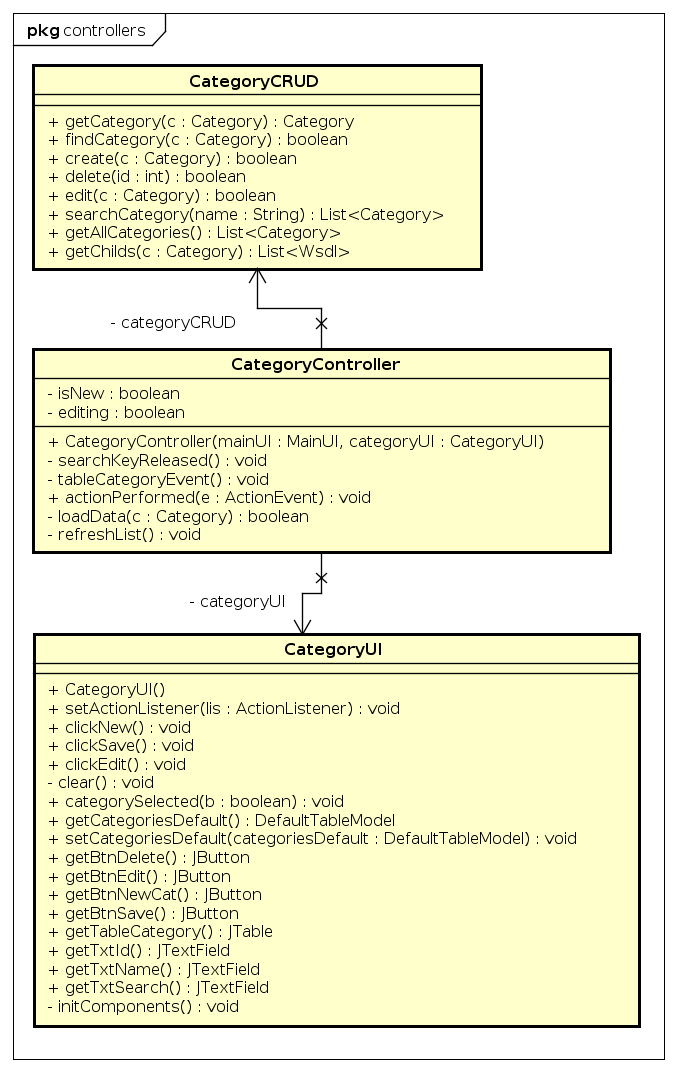
\includegraphics [scale=0.60]{imagenes/paquete_controllers.png}
 	\end{center}
 	\caption{Paquete controllers ejemplo Category.}
 	\label{fig:Paquete controllers ejemplo category}
 \end{figure} 


 Claramente se puede observar que CategoryUI implementa la interfaz de usuario, CategoryCrud el modelo y CategoryController el controlador.\\
 
 El diagrama de clase para WsdlCrud es similar al de CategoryCrud, solo difiere en los atributos.\\
 
 El diagrama de clases de diseño de la herramienta QVTWSInvoker ilustrado en la figura \ref{fig:Diagrama de clases general}, muestra cómo se relacionan las principales clases.\\

  \begin{figure}[H] 
  	\begin{center}
  		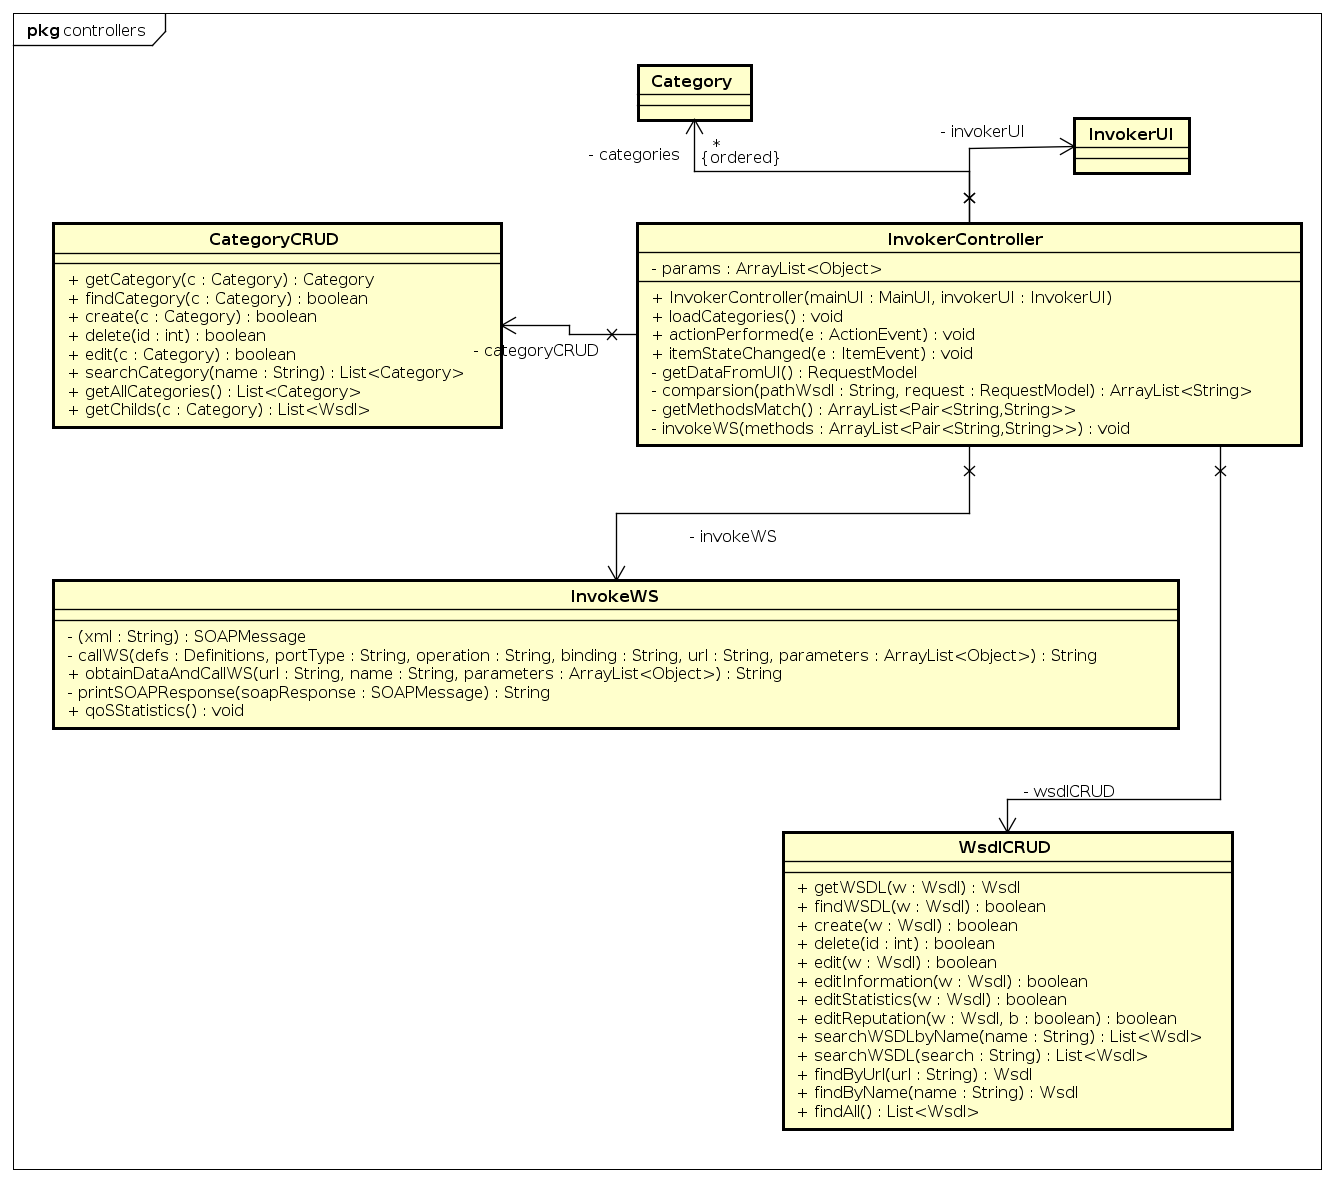
\includegraphics [scale=0.45]{imagenes/diagrama_clases_general.png}
  	\end{center}
  	\caption{Diagrama de clases general.}
  	\label{fig:Diagrama de clases general}
  \end{figure}


   En este diagrama (figura \ref{fig:Diagrama de clases general}) se puede observar que las clases InvokeWS y InvokerController son las más importantes. \\
  La clase InvokeController es la encargada de obtener la petición desde la interfaz de usuario, para luego obtener los wsdl de la categoría elegida a través del CRUD wsdlCRUD. Una vez que se tienen los wsdl y se le realiza la transformación QVT y obtención del mejor WS, se pasa a la etapa de ejecución del método del wsdl. Para ello, se utiliza la clase InvokeWS, esta fue construida con la ayuda de la librería SOA\_Distribution la cual permite automatizar la invocación a un método SOAP, una vez invocado, el resultado es mostrado por la interfaz de usuario a través del controlador InvokerController.
  
  \subsection{Modelo de Persistencia}
  
  El diagrama de clases persistentes de la herramienta QVTWSInvoker se muestra en la figura \ref{fig:Modelo persistente de la herramienta QVTWSInvoker}. Este conjunto de clases es responsable de almacenar la información de los WS's por cada ejecución. \\
  
  \begin{figure}[!h] 
  	\begin{center}
  		\includegraphics [scale=0.45]{imagenes/modelo_persistente.png}
  	\end{center}
  	\caption{Modelo persistente de la herramienta QVTWSInvoker.}
  	\label{fig:Modelo persistente de la herramienta QVTWSInvoker}
  \end{figure}
  
  A continuación se describen las tablas de la figura:\\
  
  La tabla Category representa las categorías de los WS's, tiene un identificador que es clave y un nombre, por su parte, la tabla Wsdl se encarga de mantener la información sintáctica básica de cualquier wsdl: identificador, nombre, url y categoría, además de guardar la información respecto a su calidad de servicio (reputación, tiempo de respuesta y disponibilidad).\\
  
  
\section{Herramientas utilizadas}
  
En esta sección se describen las diferentes herramientas y tecnologías utilizadas para el desarrollo de este proyecto:\\

\textbf{NetBeans y Eclipse IDE} son entornos de desarrollo integrado, que proporcionan servicios integrales para facilitarle al desarrollador o programador el desarrollo de software. Normalmente, un IDE consiste de un editor de código fuente, herramientas de construcción automáticas y un depurador.\\

\textbf{Java 1.8} es un lenguaje de programación orientado a objetos que pertenece a la empresa Sun Microsystems. Entre sus características podemos nombrar: simple, distribuido, robusto, portable, interpretado, multitareas. Se utilizó como lenguaje de programación base dentro de la herramienta NetBeans.\\

\textbf{GlassFish} es un servidor de aplicaciones de software libre desarrollado por Sun Microsystems, que implementa las tecnologías definidas en la plataforma Java EE y permite ejecutar aplicaciones que siguen esta especificación. Es gratuito y de código libre, se distribuye bajo un licenciamiento dual a través de la licencia CDDL y la GNU GPL.\\

\textbf{H2} es un sistema administrador de bases de datos relacionales programado en Java. Una de las características más importantes de H2 es que se puede integrar completamente en aplicaciones Java y acceder a la base de datos lanzando SQL directamente, sin tener que pasar por una conexión a través de sockets. Está disponible como software de código libre bajo la Licencia Pública de Mozilla o la Eclipse Public License.\\

\textbf{Eclipse Modeling Tools} contiene marcos de trabajos y herramientas para trabajar con modelos: Un modelador gráfico de Ecore, utilidad de generación de código Java para aplicaciones RCP y el marco de trabajo EMF, soporte para comparación de modelos, para esquemas XSD, OCL y modeladores gráficos en tiempo de ejecución.    
\chapter{Conclusiones y trabajos futuros}
\label{Conclusiones y trabajos futuros}

\section{Conclusiones}


En la actualidad la automatización de los procesos de negocios (Workflows) se ha convertido en un objetivo primordial para el crecimiento y desarrollo de las organizaciones. El conflicto de hoy en día a fin orden de lograr una plena automatización de los procesos, radica en la comunicación de los mismos. Y es en este sentido que la interfaz 3 de un Workflow, la de Invocación de Aplicaciones Externas, toma preponderante significado e importancia. Por ello, en función de aportar una significativa mejoría a esta comunicación, esta tesis ha llevado a cabo las siguientes propuestas expuestas con detalle a lo largo de los capítulos anteriores:

\begin{itemize}
	\item El uso del programa no solo como parte de la Interfaz de las Aplicaciones Invocadas de los WFMS, sino como un módulo externo a cualquier sistema capaz de manipular y automatizar la selección del servicio más optimo.
	\item La definición y automatización de un método de búsqueda, selección, ejecución e interpretación de resultados de WS ya conocidos.
	\item La incorporación de modelos Ecore, la transformación de modelos QVT y la medición de las QoS para describir los aspectos no funcionales de los WS's y con ello la optimización de las invocaciones externas a un Workflow en cuanto a este tipo de aplicaciones.	
	\item La aplicación e implementación de todo lo propuesto a un caso de estudio concreto.
\end{itemize}

Por otro lado, la utilización de WS's en el contexto de la Interfaz de Aplicaciones Invocadas, tiene el principal beneficio o ventaja de aprovechar la información disponible en la web a través de éstos, es decir, tener la posibilidad de que las aplicaciones externas al WFMS estén distribuidas en la red, en cualquier parte del mundo, y que ello resulte completamente transparente al WFMS, e incluso al motor del mismo. Así se fundamenta que tanto la búsqueda, como la selección y la ejecución de estas aplicaciones previamente conocidas, se realice de forma dinámica y automática.\\
Otra contribución importante de esta tesis es la optimización de la invocación (y con ello la comunicación) entre un WFMS y las aplicaciones con quienes debe interactuar. Esta optimización consiste en tener en cuenta a la hora de la selección de aplicaciones los atributos no funcionales, o QoS, de los WS's. Ello permite compartir recursos distribuidos a gran escala, lo cual puede implicar por ejemplo la integración entre Workflows.
El uso de WS's plantea una forma unificada de acceder a las aplicaciones. Este acceso posibilita la interacción con servicios y/o métodos comunes favoreciendo la interoperabilidad a través de las diferentes plataformas. Existen numerosas ventajas que benefician la distribución de las aplicaciones y la interoperabilidad de los sistemas al utilizar este tipo de aplicaciones, dado que permiten la utilización de aplicaciones de componentes abiertas y auto descriptas, la composición rápida de aplicaciones distribuidas, el uso de aplicaciones modulares y desacopladas, la independencia de la plataforma subyacente y el lenguaje de programación, el acoplamiento débil, etc.\\

Por todas estas razones es que se convierten en un excelente recurso para permitir la distribución transparente de las aplicaciones externas a los WFMS.

\section{Trabajos Futuros}

A continuación se enumeran las posibles extensiones para este trabajo:\\

En primer lugar, se considera importante que la herramienta otorgue diferentes posibilidades en cuanto a la selección de las QoS deseadas en la aplicación que se quiera buscar. Resulta muy interesante ampliar este espectro y así permitir al usuario de la herramienta escoger entre un conjunto más amplio de QoS.\\

También es necesario que la herramienta sea apta para manipular intercambio de mensajes REST, debido al gran auge que están teniendo, y así dar la posibilidad de que esta comunicación no se realice únicamente a través del protocolo SOAP.\\

Al mismo tiempo, la herramienta necesita el uso de la plantilla de salida estándar para desligar al usuario de la responsabilidad de interpretar las diferentes sintaxis de los resultados obtenidos. Esto no solo reduciría la complejidad que implica implementar en un Workflow la interfaz de invocación de aplicaciones, sino que también logra estandarizar el resultado para cualquier tipo de WS especificado.\\

Una variante a lo propuesto en este trabajo, es el hecho de utilizar procesamiento del lenguaje a la hora de hacer la comparación de modelos y así poder utilizar otra información, como por ejemplo la descripción. 

%% This defines the bibliography file (main.bib) and the bibliography style.
%% If you want to create a bibliography file by hand, change the contents of
%% this file to a `thebibliography' environment.  For more information 
%% see section 4.3 of the LaTeX manual.

\bibliography{bibliografia}
\bibliographystyle{plain}


\chapter*{Apéndices}
\label{Apendices}
\markboth{Apendices}{} % para que cambie el encabezado, si no, usaría el del último chapter{}
\addcontentsline{toc}{chapter}{Apéndices} % para que se añada en el indice

\appendix
\chapter{Especificación de la Transformación en Query/View/Transformation Relations}
\label{Especificacion de la Transformacion en QVT/Relations QVT}


%\section{Especificación de la Transformación en QVT/ Relations QVT}
%\label{Especificación de la Transformación en QVT/Relations QVT}
Código completo, en QVT Relation, de la transformación de máquinas de estados con elementos opcionales a máquinas de estados concretas.

\begin{verbatim}
-- Inicio de la Transformación 

\end{verbatim}


\printindex

\end{document}